\documentclass{book}
\usepackage[a4paper,top=2.5cm,bottom=2.5cm,left=2.5cm,right=2.5cm]{geometry}
\usepackage{makeidx}
\usepackage{natbib}
\usepackage{graphicx}
\usepackage{multicol}
\usepackage{float}
\usepackage{listings}
\usepackage{color}
\usepackage{ifthen}
\usepackage[table]{xcolor}
\usepackage{textcomp}
\usepackage{alltt}
\usepackage{ifpdf}
\ifpdf
\usepackage[pdftex,
            pagebackref=true,
            colorlinks=true,
            linkcolor=blue,
            unicode
           ]{hyperref}
\else
\usepackage[ps2pdf,
            pagebackref=true,
            colorlinks=true,
            linkcolor=blue,
            unicode
           ]{hyperref}
\usepackage{pspicture}
\fi
\usepackage[utf8]{inputenc}
\usepackage{mathptmx}
\usepackage[scaled=.90]{helvet}
\usepackage{courier}
\usepackage{sectsty}
\usepackage[titles]{tocloft}
\usepackage{doxygen}
\lstset{language=C++,inputencoding=utf8,basicstyle=\footnotesize,breaklines=true,breakatwhitespace=true,tabsize=8,numbers=left }
\makeindex
\setcounter{tocdepth}{3}
\renewcommand{\footrulewidth}{0.4pt}
\renewcommand{\familydefault}{\sfdefault}
\hfuzz=15pt
\setlength{\emergencystretch}{15pt}
\hbadness=750
\tolerance=750
\begin{document}
\hypersetup{pageanchor=false,citecolor=blue}
\begin{titlepage}
\vspace*{7cm}
\begin{center}
{\Large Projet Calculatrice à notation polonaise inversée \\[1ex]\large 3\-\_\-1 }\\
\vspace*{1cm}
{\large Generated by Doxygen 1.8.1.1}\\
\vspace*{0.5cm}
{\small Sun Jun 17 2012 11:34:32}\\
\end{center}
\end{titlepage}
\clearemptydoublepage
\pagenumbering{roman}
\tableofcontents
\clearemptydoublepage
\pagenumbering{arabic}
\hypersetup{pageanchor=true,citecolor=blue}
\chapter{Class Index}
\section{Hiérarchie des classes}
Cette liste d'héritage est classée approximativement par ordre alphabétique \-:\begin{DoxyCompactList}
\item \contentsline{section}{Calculatrice\-Modele}{\pageref{class_calculatrice_modele}}{}
\item \contentsline{section}{Calcul\-:\-:Constante}{\pageref{class_calcul_1_1_constante}}{}
\begin{DoxyCompactList}
\item \contentsline{section}{Calcul\-:\-:Complexe}{\pageref{class_calcul_1_1_complexe}}{}
\item \contentsline{section}{Calcul\-:\-:Expression}{\pageref{class_calcul_1_1_expression}}{}
\item \contentsline{section}{Calcul\-:\-:Nombre}{\pageref{class_calcul_1_1_nombre}}{}
\begin{DoxyCompactList}
\item \contentsline{section}{Calcul\-:\-:Entier}{\pageref{class_calcul_1_1_entier}}{}
\item \contentsline{section}{Calcul\-:\-:Rationnel}{\pageref{class_calcul_1_1_rationnel}}{}
\item \contentsline{section}{Calcul\-:\-:Reel}{\pageref{class_calcul_1_1_reel}}{}
\end{DoxyCompactList}
\end{DoxyCompactList}
\item \contentsline{section}{Fabrique\-Constante}{\pageref{class_fabrique_constante}}{}
\item \contentsline{section}{Fabrique\-Nombre}{\pageref{class_fabrique_nombre}}{}
\item \contentsline{section}{Stack\-:\-:iterator}{\pageref{class_stack_1_1iterator}}{}
\item \contentsline{section}{Logger}{\pageref{class_logger}}{}
\begin{DoxyCompactList}
\item \contentsline{section}{Logger\-Console}{\pageref{class_logger_console}}{}
\item \contentsline{section}{Logger\-File}{\pageref{class_logger_file}}{}
\end{DoxyCompactList}
\item \contentsline{section}{Log\-Message}{\pageref{class_log_message}}{}
\item \contentsline{section}{Main\-Window}{\pageref{class_main_window}}{}
\item \contentsline{section}{Stack}{\pageref{class_stack}}{}
\end{DoxyCompactList}

\chapter{Class Index}
\section{Class List}
Here are the classes, structs, unions and interfaces with brief descriptions\-:\begin{DoxyCompactList}
\item\contentsline{section}{\hyperlink{class_calculatrice_modele}{Calculatrice\-Modele} }{\pageref{class_calculatrice_modele}}{}
\item\contentsline{section}{\hyperlink{class_calcul_1_1_complexe}{Calcul\-::\-Complexe} }{\pageref{class_calcul_1_1_complexe}}{}
\item\contentsline{section}{\hyperlink{class_calcul_1_1_constante}{Calcul\-::\-Constante} }{\pageref{class_calcul_1_1_constante}}{}
\item\contentsline{section}{\hyperlink{class_calcul_1_1_entier}{Calcul\-::\-Entier} }{\pageref{class_calcul_1_1_entier}}{}
\item\contentsline{section}{\hyperlink{class_calcul_1_1_expression}{Calcul\-::\-Expression} }{\pageref{class_calcul_1_1_expression}}{}
\item\contentsline{section}{\hyperlink{class_fabrique_constante}{Fabrique\-Constante} }{\pageref{class_fabrique_constante}}{}
\item\contentsline{section}{\hyperlink{class_fabrique_nombre}{Fabrique\-Nombre} }{\pageref{class_fabrique_nombre}}{}
\item\contentsline{section}{\hyperlink{class_main_window}{Main\-Window} }{\pageref{class_main_window}}{}
\item\contentsline{section}{\hyperlink{class_calcul_1_1_nombre}{Calcul\-::\-Nombre} }{\pageref{class_calcul_1_1_nombre}}{}
\item\contentsline{section}{\hyperlink{class_calcul_1_1_rationnel}{Calcul\-::\-Rationnel} }{\pageref{class_calcul_1_1_rationnel}}{}
\item\contentsline{section}{\hyperlink{class_calcul_1_1_reel}{Calcul\-::\-Reel} }{\pageref{class_calcul_1_1_reel}}{}
\item\contentsline{section}{\hyperlink{class_stack}{Stack} }{\pageref{class_stack}}{}
\end{DoxyCompactList}

\chapter{File Index}
\section{File List}
Here is a list of all documented files with brief descriptions\-:\begin{DoxyCompactList}
\item\contentsline{section}{\hyperlink{_calculatrice_modele_8h}{Calculatrice\-Modele.\-h} \\*G�re la calculatrice }{\pageref{_calculatrice_modele_8h}}{}
\item\contentsline{section}{{\bfseries Constante\-\_\-\-Factory.\-h} }{\pageref{_constante___factory_8h}}{}
\item\contentsline{section}{{\bfseries Constantes.\-h} }{\pageref{_constantes_8h}}{}
\item\contentsline{section}{{\bfseries Gestion\-\_\-constantes.\-h} }{\pageref{_gestion__constantes_8h}}{}
\item\contentsline{section}{{\bfseries mainwindow.\-h} }{\pageref{mainwindow_8h}}{}
\end{DoxyCompactList}

\chapter{Class Documentation}
\hypertarget{class_calculatrice_modele}{\section{Calculatrice\-Modele Class Reference}
\label{class_calculatrice_modele}\index{Calculatrice\-Modele@{Calculatrice\-Modele}}
}
\subsection*{Public Slots}
\begin{DoxyCompactItemize}
\item 
\hypertarget{class_calculatrice_modele_a2214a44a1baedaaa580520967595b224}{void {\bfseries get\-Nombre} (Q\-String s, bool complexe)}\label{class_calculatrice_modele_a2214a44a1baedaaa580520967595b224}

\item 
\hypertarget{class_calculatrice_modele_a381382f5fb175a17915a057009051d4a}{void {\bfseries get\-Expression} ()}\label{class_calculatrice_modele_a381382f5fb175a17915a057009051d4a}

\item 
\hypertarget{class_calculatrice_modele_a607d33dc6cf27f3a6720b16d1891627a}{void {\bfseries get\-Add} ()}\label{class_calculatrice_modele_a607d33dc6cf27f3a6720b16d1891627a}

\item 
\hypertarget{class_calculatrice_modele_ac545a816c1ff8e79f178e17819b6b0c4}{void {\bfseries get\-Sous} ()}\label{class_calculatrice_modele_ac545a816c1ff8e79f178e17819b6b0c4}

\item 
\hypertarget{class_calculatrice_modele_a5865e8e444be2412ef587d5bd95384d3}{void {\bfseries get\-Mult} ()}\label{class_calculatrice_modele_a5865e8e444be2412ef587d5bd95384d3}

\item 
\hypertarget{class_calculatrice_modele_a61acc0db8a62c2b920b8f430231e1d2e}{void {\bfseries get\-Div} (int type)}\label{class_calculatrice_modele_a61acc0db8a62c2b920b8f430231e1d2e}

\item 
\hypertarget{class_calculatrice_modele_a96b09c72f026835a32fabed8777124e2}{void {\bfseries get\-Pow} ()}\label{class_calculatrice_modele_a96b09c72f026835a32fabed8777124e2}

\item 
\hypertarget{class_calculatrice_modele_aeb7d0373268778e2b0e4dc52bef66a76}{void {\bfseries get\-Mod} ()}\label{class_calculatrice_modele_aeb7d0373268778e2b0e4dc52bef66a76}

\item 
\hypertarget{class_calculatrice_modele_a49279e61204e623526d0f66ba8bf26bb}{void {\bfseries get\-Fact} ()}\label{class_calculatrice_modele_a49279e61204e623526d0f66ba8bf26bb}

\item 
\hypertarget{class_calculatrice_modele_a962573381f42a5dfac301bc5213619ce}{void {\bfseries get\-Sign} ()}\label{class_calculatrice_modele_a962573381f42a5dfac301bc5213619ce}

\item 
\hypertarget{class_calculatrice_modele_af0cecf65dd551eeb9c0f13828c0e0f8c}{void {\bfseries get\-Sin} (bool degre)}\label{class_calculatrice_modele_af0cecf65dd551eeb9c0f13828c0e0f8c}

\item 
\hypertarget{class_calculatrice_modele_a5c14279e32094874effeed4a9260a2fa}{void {\bfseries get\-Cos} (bool degre)}\label{class_calculatrice_modele_a5c14279e32094874effeed4a9260a2fa}

\item 
\hypertarget{class_calculatrice_modele_af3231b806c518b0f028906cd5d47c3ed}{void {\bfseries get\-Tan} (bool degre)}\label{class_calculatrice_modele_af3231b806c518b0f028906cd5d47c3ed}

\item 
\hypertarget{class_calculatrice_modele_a8907fc8b58dcc77324a30a0775e70ca2}{void {\bfseries get\-Sinh} (bool degre)}\label{class_calculatrice_modele_a8907fc8b58dcc77324a30a0775e70ca2}

\item 
\hypertarget{class_calculatrice_modele_ac7e58e32ba5ab4da8e8fea5ed6c71d13}{void {\bfseries get\-Cosh} (bool degre)}\label{class_calculatrice_modele_ac7e58e32ba5ab4da8e8fea5ed6c71d13}

\item 
\hypertarget{class_calculatrice_modele_a22595921ae15989ff22245b0d1575c10}{void {\bfseries get\-Tanh} (bool degre)}\label{class_calculatrice_modele_a22595921ae15989ff22245b0d1575c10}

\item 
\hypertarget{class_calculatrice_modele_ad155cab2b58ac17e026d48a15a40c562}{void {\bfseries get\-Ln} ()}\label{class_calculatrice_modele_ad155cab2b58ac17e026d48a15a40c562}

\item 
\hypertarget{class_calculatrice_modele_a657b0a941efaf0f43d1f585cd98acfe1}{void {\bfseries get\-Log} ()}\label{class_calculatrice_modele_a657b0a941efaf0f43d1f585cd98acfe1}

\item 
\hypertarget{class_calculatrice_modele_a923629b6b9c478d23d45392e5682e731}{void {\bfseries get\-Inv} ()}\label{class_calculatrice_modele_a923629b6b9c478d23d45392e5682e731}

\item 
\hypertarget{class_calculatrice_modele_addcc1a83cd24dd180d295c46ca489b42}{void {\bfseries get\-Sqrt} ()}\label{class_calculatrice_modele_addcc1a83cd24dd180d295c46ca489b42}

\item 
\hypertarget{class_calculatrice_modele_a79b4a04f15a6b6ba53f8a9d4ab99ee97}{void {\bfseries get\-Sqr} ()}\label{class_calculatrice_modele_a79b4a04f15a6b6ba53f8a9d4ab99ee97}

\item 
\hypertarget{class_calculatrice_modele_a35f825314f6eb60c3f43237b6add63a0}{void {\bfseries get\-Cube} ()}\label{class_calculatrice_modele_a35f825314f6eb60c3f43237b6add63a0}

\item 
\hypertarget{class_calculatrice_modele_ac22ca78efd8da136c6c823052a1b4288}{void {\bfseries get\-Swap} ()}\label{class_calculatrice_modele_ac22ca78efd8da136c6c823052a1b4288}

\item 
\hypertarget{class_calculatrice_modele_acbc58d1fb5d6b0864808b9fe4e004943}{void {\bfseries get\-Sum} ()}\label{class_calculatrice_modele_acbc58d1fb5d6b0864808b9fe4e004943}

\item 
\hypertarget{class_calculatrice_modele_a55634029d3d7bcdb7dc3994c6d00270f}{void {\bfseries get\-Mean} ()}\label{class_calculatrice_modele_a55634029d3d7bcdb7dc3994c6d00270f}

\item 
\hypertarget{class_calculatrice_modele_a8fa5323fa79c861c76453b70a4ca9c9b}{void {\bfseries get\-Clear} ()}\label{class_calculatrice_modele_a8fa5323fa79c861c76453b70a4ca9c9b}

\item 
\hypertarget{class_calculatrice_modele_a5b6d0f57fa7c4b271ef296ea587d7b14}{void {\bfseries get\-Dup} ()}\label{class_calculatrice_modele_a5b6d0f57fa7c4b271ef296ea587d7b14}

\item 
\hypertarget{class_calculatrice_modele_a7230f86783c54d8c7d609086059fc676}{void {\bfseries get\-Drop} ()}\label{class_calculatrice_modele_a7230f86783c54d8c7d609086059fc676}

\end{DoxyCompactItemize}
\subsection*{Signals}
\begin{DoxyCompactItemize}
\item 
\hypertarget{class_calculatrice_modele_a491b838119e11d843a5b7ae9ed1d3c9c}{void {\bfseries fin\-Op} (\hyperlink{class_calcul_1_1_constante}{Constante} $\ast$cte, int i)}\label{class_calculatrice_modele_a491b838119e11d843a5b7ae9ed1d3c9c}

\item 
\hypertarget{class_calculatrice_modele_ad741ddfdf7320455e53b0499bd9ec6b6}{void {\bfseries eval\-Exp} (Q\-String s)}\label{class_calculatrice_modele_ad741ddfdf7320455e53b0499bd9ec6b6}

\end{DoxyCompactItemize}
\subsection*{Public Member Functions}
\begin{DoxyCompactItemize}
\item 
\hypertarget{class_calculatrice_modele_acdb374ef7094036d07dfd59241674a7c}{{\bfseries Calculatrice\-Modele} (Q\-Object $\ast$parent=0)}\label{class_calculatrice_modele_acdb374ef7094036d07dfd59241674a7c}

\item 
\hypertarget{class_calculatrice_modele_ae311466b783cc6418efeaef854df461a}{void {\bfseries affiche\-Pile\-Taille} ()}\label{class_calculatrice_modele_ae311466b783cc6418efeaef854df461a}

\end{DoxyCompactItemize}


The documentation for this class was generated from the following files\-:\begin{DoxyCompactItemize}
\item 
\hyperlink{_calculatrice_modele_8h}{Calculatrice\-Modele.\-h}\item 
Calculatrice\-Modele.\-cpp\end{DoxyCompactItemize}

\hypertarget{class_calcul_1_1_complexe}{\section{Référence de la classe Calcul\-:\-:Complexe}
\label{class_calcul_1_1_complexe}\index{Calcul\-::\-Complexe@{Calcul\-::\-Complexe}}
}


Classe qui contiendra deux pointeurs vers des objets de type \hyperlink{class_calcul_1_1_nombre}{Nombre}.  




{\ttfamily \#include $<$Constantes.\-h$>$}

Graphe d'héritage de Calcul\-:\-:Complexe\-:\begin{figure}[H]
\begin{center}
\leavevmode
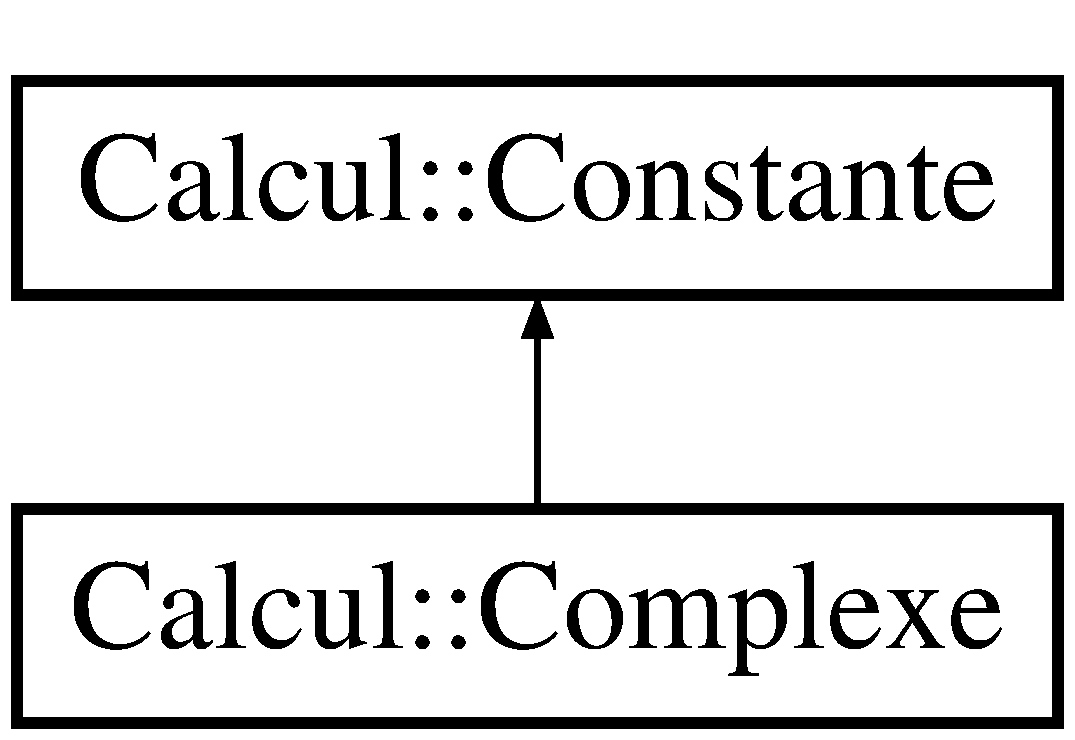
\includegraphics[height=2.000000cm]{class_calcul_1_1_complexe}
\end{center}
\end{figure}
\subsection*{Fonctions membres publiques}
\begin{DoxyCompactItemize}
\item 
\hypertarget{class_calcul_1_1_complexe_a339a3e1127659228bb342a3e83433927}{{\bfseries Complexe} (Q\-String s=\char`\"{}0\$0\char`\"{})}\label{class_calcul_1_1_complexe_a339a3e1127659228bb342a3e83433927}

\item 
\hypertarget{class_calcul_1_1_complexe_ad47a4a48e44aa777f6e598f8221dea42}{{\bfseries Complexe} (\hyperlink{class_calcul_1_1_nombre}{Nombre} $\ast$reel, \hyperlink{class_calcul_1_1_nombre}{Nombre} $\ast$imaginaire=N\-U\-L\-L)}\label{class_calcul_1_1_complexe_ad47a4a48e44aa777f6e598f8221dea42}

\item 
\hypertarget{class_calcul_1_1_complexe_a042ce33da08cb71e717ac3b67e6c964b}{{\bfseries Complexe} (\hyperlink{class_calcul_1_1_complexe}{Complexe} $\ast$comp)}\label{class_calcul_1_1_complexe_a042ce33da08cb71e717ac3b67e6c964b}

\item 
\hypertarget{class_calcul_1_1_complexe_acb9136f710db8d1d83a5a25d76fb6dfe}{\hyperlink{class_calcul_1_1_nombre}{Nombre} $\ast$ {\bfseries Get\-Re} () const }\label{class_calcul_1_1_complexe_acb9136f710db8d1d83a5a25d76fb6dfe}

\item 
\hypertarget{class_calcul_1_1_complexe_a07757377f6a1de6afd6364edb00784b7}{\hyperlink{class_calcul_1_1_nombre}{Nombre} $\ast$ {\bfseries Get\-Im} () const }\label{class_calcul_1_1_complexe_a07757377f6a1de6afd6364edb00784b7}

\item 
\hypertarget{class_calcul_1_1_complexe_af544268718f1709a2ff534210051442c}{void {\bfseries Set\-Re} (\hyperlink{class_calcul_1_1_nombre}{Nombre} $\ast$r)}\label{class_calcul_1_1_complexe_af544268718f1709a2ff534210051442c}

\item 
\hypertarget{class_calcul_1_1_complexe_a14ba5f590705435810d24d29e59b1012}{void {\bfseries Set\-Im} (\hyperlink{class_calcul_1_1_nombre}{Nombre} $\ast$i)}\label{class_calcul_1_1_complexe_a14ba5f590705435810d24d29e59b1012}

\item 
\hypertarget{class_calcul_1_1_complexe_a2e153caf21e98a21ccbd02ed55896056}{bool {\bfseries is\-Null} ()}\label{class_calcul_1_1_complexe_a2e153caf21e98a21ccbd02ed55896056}

\item 
const Q\-String \hyperlink{class_calcul_1_1_complexe_a3f444d3a18104aeb6f1490c0d3a57e6d}{Convert\-Chaine} () const 
\begin{DoxyCompactList}\small\item\em Convert\-Chaine Méthode virtuelle qui convertit une \hyperlink{class_calcul_1_1_constante}{Constante} en une chaine de caractères. \end{DoxyCompactList}\item 
\hypertarget{class_calcul_1_1_complexe_ac94d8bd297d11ca9c6be59ff1de8fbe3}{\hyperlink{class_calcul_1_1_complexe}{Complexe} {\bfseries operator+} (\hyperlink{class_calcul_1_1_complexe}{Complexe} r1)}\label{class_calcul_1_1_complexe_ac94d8bd297d11ca9c6be59ff1de8fbe3}

\item 
\hypertarget{class_calcul_1_1_complexe_a492d158468de2f7f221957781e4626a7}{\hyperlink{class_calcul_1_1_complexe}{Complexe} {\bfseries operator+} (\hyperlink{class_calcul_1_1_entier}{Entier} r1)}\label{class_calcul_1_1_complexe_a492d158468de2f7f221957781e4626a7}

\item 
\hypertarget{class_calcul_1_1_complexe_aad76bb715ecea3ce33eeab06ec3d7440}{\hyperlink{class_calcul_1_1_complexe}{Complexe} {\bfseries operator+} (\hyperlink{class_calcul_1_1_reel}{Reel} r1)}\label{class_calcul_1_1_complexe_aad76bb715ecea3ce33eeab06ec3d7440}

\item 
\hypertarget{class_calcul_1_1_complexe_adfeffbd2a63dfc4b49647ddc92bc9282}{\hyperlink{class_calcul_1_1_complexe}{Complexe} {\bfseries operator+} (\hyperlink{class_calcul_1_1_rationnel}{Rationnel} r1)}\label{class_calcul_1_1_complexe_adfeffbd2a63dfc4b49647ddc92bc9282}

\item 
\hypertarget{class_calcul_1_1_complexe_aa0902e9e1ca9fbc3b180ecc327bf793b}{\hyperlink{class_calcul_1_1_constante}{Constante} $\ast$ {\bfseries operator+} (\hyperlink{class_calcul_1_1_constante}{Constante} $\ast$r1)}\label{class_calcul_1_1_complexe_aa0902e9e1ca9fbc3b180ecc327bf793b}

\item 
\hypertarget{class_calcul_1_1_complexe_a8693b425a124816514a4d8eeded47f98}{\hyperlink{class_calcul_1_1_complexe}{Complexe} {\bfseries operator-\/} (\hyperlink{class_calcul_1_1_complexe}{Complexe} r1)}\label{class_calcul_1_1_complexe_a8693b425a124816514a4d8eeded47f98}

\item 
\hypertarget{class_calcul_1_1_complexe_aa10f5be965f69957eaf7096f99999d53}{\hyperlink{class_calcul_1_1_complexe}{Complexe} {\bfseries operator-\/} ()}\label{class_calcul_1_1_complexe_aa10f5be965f69957eaf7096f99999d53}

\item 
\hypertarget{class_calcul_1_1_complexe_a5e2bc169c73cf545bf877281fe334cbc}{\hyperlink{class_calcul_1_1_complexe}{Complexe} {\bfseries operator-\/} (\hyperlink{class_calcul_1_1_entier}{Entier} r1)}\label{class_calcul_1_1_complexe_a5e2bc169c73cf545bf877281fe334cbc}

\item 
\hypertarget{class_calcul_1_1_complexe_a6c63acf2cd345464795836ddcb8738fd}{\hyperlink{class_calcul_1_1_complexe}{Complexe} {\bfseries operator-\/} (\hyperlink{class_calcul_1_1_reel}{Reel} r1)}\label{class_calcul_1_1_complexe_a6c63acf2cd345464795836ddcb8738fd}

\item 
\hypertarget{class_calcul_1_1_complexe_ae5589111d6416e47e41e9c3b8dcc1c9f}{\hyperlink{class_calcul_1_1_complexe}{Complexe} {\bfseries operator-\/} (\hyperlink{class_calcul_1_1_rationnel}{Rationnel} r1)}\label{class_calcul_1_1_complexe_ae5589111d6416e47e41e9c3b8dcc1c9f}

\item 
\hypertarget{class_calcul_1_1_complexe_a8ef9beccece877eef7bc6a1556fc6d0a}{\hyperlink{class_calcul_1_1_constante}{Constante} $\ast$ {\bfseries operator-\/} (\hyperlink{class_calcul_1_1_constante}{Constante} $\ast$r1)}\label{class_calcul_1_1_complexe_a8ef9beccece877eef7bc6a1556fc6d0a}

\item 
\hypertarget{class_calcul_1_1_complexe_a73137718dd47663a1a16636e9efbf839}{\hyperlink{class_calcul_1_1_complexe}{Complexe} {\bfseries operator$\ast$} (\hyperlink{class_calcul_1_1_complexe}{Complexe} r1)}\label{class_calcul_1_1_complexe_a73137718dd47663a1a16636e9efbf839}

\item 
\hypertarget{class_calcul_1_1_complexe_a3c6be886ae5dab4d10c3d8b1efb16409}{\hyperlink{class_calcul_1_1_complexe}{Complexe} {\bfseries operator$\ast$} (\hyperlink{class_calcul_1_1_entier}{Entier} r1)}\label{class_calcul_1_1_complexe_a3c6be886ae5dab4d10c3d8b1efb16409}

\item 
\hypertarget{class_calcul_1_1_complexe_a31bb611985dca4960ba6618ba0728323}{\hyperlink{class_calcul_1_1_complexe}{Complexe} {\bfseries operator$\ast$} (\hyperlink{class_calcul_1_1_reel}{Reel} r1)}\label{class_calcul_1_1_complexe_a31bb611985dca4960ba6618ba0728323}

\item 
\hypertarget{class_calcul_1_1_complexe_acbab16bac207e911f3637c1fb5a5ca31}{\hyperlink{class_calcul_1_1_complexe}{Complexe} {\bfseries operator$\ast$} (\hyperlink{class_calcul_1_1_rationnel}{Rationnel} r1)}\label{class_calcul_1_1_complexe_acbab16bac207e911f3637c1fb5a5ca31}

\item 
\hypertarget{class_calcul_1_1_complexe_a498db39ecf1dc24954cd5b47323f9798}{\hyperlink{class_calcul_1_1_constante}{Constante} $\ast$ {\bfseries operator$\ast$} (\hyperlink{class_calcul_1_1_constante}{Constante} $\ast$r1)}\label{class_calcul_1_1_complexe_a498db39ecf1dc24954cd5b47323f9798}

\item 
\hypertarget{class_calcul_1_1_complexe_ad43d455f0c78e8c8286718a53770716d}{\hyperlink{class_calcul_1_1_complexe}{Complexe} {\bfseries operator/} (\hyperlink{class_calcul_1_1_complexe}{Complexe} r1)}\label{class_calcul_1_1_complexe_ad43d455f0c78e8c8286718a53770716d}

\item 
\hypertarget{class_calcul_1_1_complexe_a30bb25d0dc2d4682b41d1fa75e1e9b9d}{\hyperlink{class_calcul_1_1_complexe}{Complexe} {\bfseries operator/} (\hyperlink{class_calcul_1_1_entier}{Entier} r1)}\label{class_calcul_1_1_complexe_a30bb25d0dc2d4682b41d1fa75e1e9b9d}

\item 
\hypertarget{class_calcul_1_1_complexe_aeda42f5c908477ce344afdef2b979f5b}{\hyperlink{class_calcul_1_1_complexe}{Complexe} {\bfseries operator/} (\hyperlink{class_calcul_1_1_reel}{Reel} r1)}\label{class_calcul_1_1_complexe_aeda42f5c908477ce344afdef2b979f5b}

\item 
\hypertarget{class_calcul_1_1_complexe_a783b5949f0ed1f6a5a9b4db367ec2d72}{\hyperlink{class_calcul_1_1_complexe}{Complexe} {\bfseries operator/} (\hyperlink{class_calcul_1_1_rationnel}{Rationnel} r1)}\label{class_calcul_1_1_complexe_a783b5949f0ed1f6a5a9b4db367ec2d72}

\item 
\hypertarget{class_calcul_1_1_complexe_a9cba41b08b70e3b1f322617cf8568dd4}{\hyperlink{class_calcul_1_1_constante}{Constante} $\ast$ {\bfseries operator/} (\hyperlink{class_calcul_1_1_constante}{Constante} $\ast$r1)}\label{class_calcul_1_1_complexe_a9cba41b08b70e3b1f322617cf8568dd4}

\item 
\hypertarget{class_calcul_1_1_complexe_a0ecafe9cdd55cc5f04ea3c8316764139}{\hyperlink{class_calcul_1_1_complexe}{Complexe} {\bfseries sqr} ()}\label{class_calcul_1_1_complexe_a0ecafe9cdd55cc5f04ea3c8316764139}

\item 
\hypertarget{class_calcul_1_1_complexe_a08d3991ff3a10788c131fdf67ac4524f}{\hyperlink{class_calcul_1_1_complexe}{Complexe} {\bfseries cube} ()}\label{class_calcul_1_1_complexe_a08d3991ff3a10788c131fdf67ac4524f}

\end{DoxyCompactItemize}


\subsection{Description détaillée}
Classe qui contiendra deux pointeurs vers des objets de type \hyperlink{class_calcul_1_1_nombre}{Nombre}. 

\subsection{Documentation des fonctions membres}
\hypertarget{class_calcul_1_1_complexe_a3f444d3a18104aeb6f1490c0d3a57e6d}{\index{Calcul\-::\-Complexe@{Calcul\-::\-Complexe}!Convert\-Chaine@{Convert\-Chaine}}
\index{Convert\-Chaine@{Convert\-Chaine}!Calcul::Complexe@{Calcul\-::\-Complexe}}
\subsubsection[{Convert\-Chaine}]{\setlength{\rightskip}{0pt plus 5cm}const Q\-String Calcul\-::\-Complexe\-::\-Convert\-Chaine (
\begin{DoxyParamCaption}
{}
\end{DoxyParamCaption}
) const\hspace{0.3cm}{\ttfamily [inline]}, {\ttfamily [virtual]}}}\label{class_calcul_1_1_complexe_a3f444d3a18104aeb6f1490c0d3a57e6d}


Convert\-Chaine Méthode virtuelle qui convertit une \hyperlink{class_calcul_1_1_constante}{Constante} en une chaine de caractères. 

\begin{DoxyReturn}{Renvoie}
Retourne un const Q\-String 
\end{DoxyReturn}


Implémente \hyperlink{class_calcul_1_1_constante_a80fb461841b16e6d5d1339802b69858e}{Calcul\-::\-Constante}.



La documentation de cette classe a été générée à partir des fichiers suivants \-:\begin{DoxyCompactItemize}
\item 
Projet\-\_\-\-L\-O21\-\_\-v3\-\_\-1/\hyperlink{_constantes_8h}{Constantes.\-h}\item 
Projet\-\_\-\-L\-O21\-\_\-v3\-\_\-1/\hyperlink{_complexe_8cpp}{Complexe.\-cpp}\end{DoxyCompactItemize}

\hypertarget{class_calcul_1_1_constante}{\section{Calcul\-:\-:Constante Class Reference}
\label{class_calcul_1_1_constante}\index{Calcul\-::\-Constante@{Calcul\-::\-Constante}}
}
Inheritance diagram for Calcul\-:\-:Constante\-:\begin{figure}[H]
\begin{center}
\leavevmode
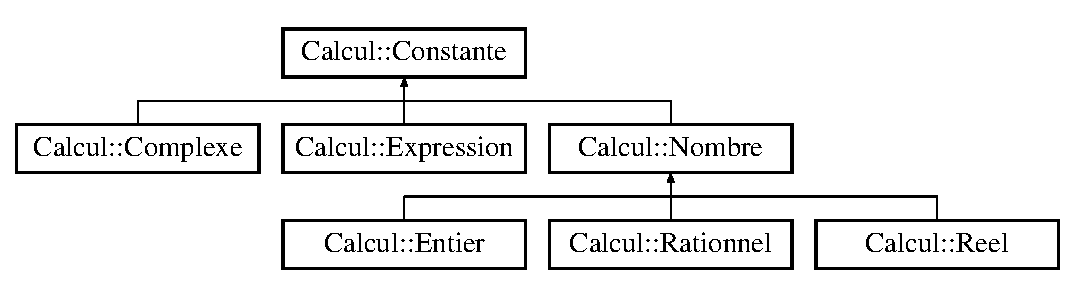
\includegraphics[height=3.000000cm]{class_calcul_1_1_constante}
\end{center}
\end{figure}
\subsection*{Public Member Functions}
\begin{DoxyCompactItemize}
\item 
\hypertarget{class_calcul_1_1_constante_a80fb461841b16e6d5d1339802b69858e}{virtual const Q\-String {\bfseries Convert\-Chaine} () const =0}\label{class_calcul_1_1_constante_a80fb461841b16e6d5d1339802b69858e}

\end{DoxyCompactItemize}


The documentation for this class was generated from the following file\-:\begin{DoxyCompactItemize}
\item 
Constantes.\-h\end{DoxyCompactItemize}

\hypertarget{class_calcul_1_1_entier}{\section{Calcul\-:\-:Entier Class Reference}
\label{class_calcul_1_1_entier}\index{Calcul\-::\-Entier@{Calcul\-::\-Entier}}
}
Inheritance diagram for Calcul\-:\-:Entier\-:\begin{figure}[H]
\begin{center}
\leavevmode
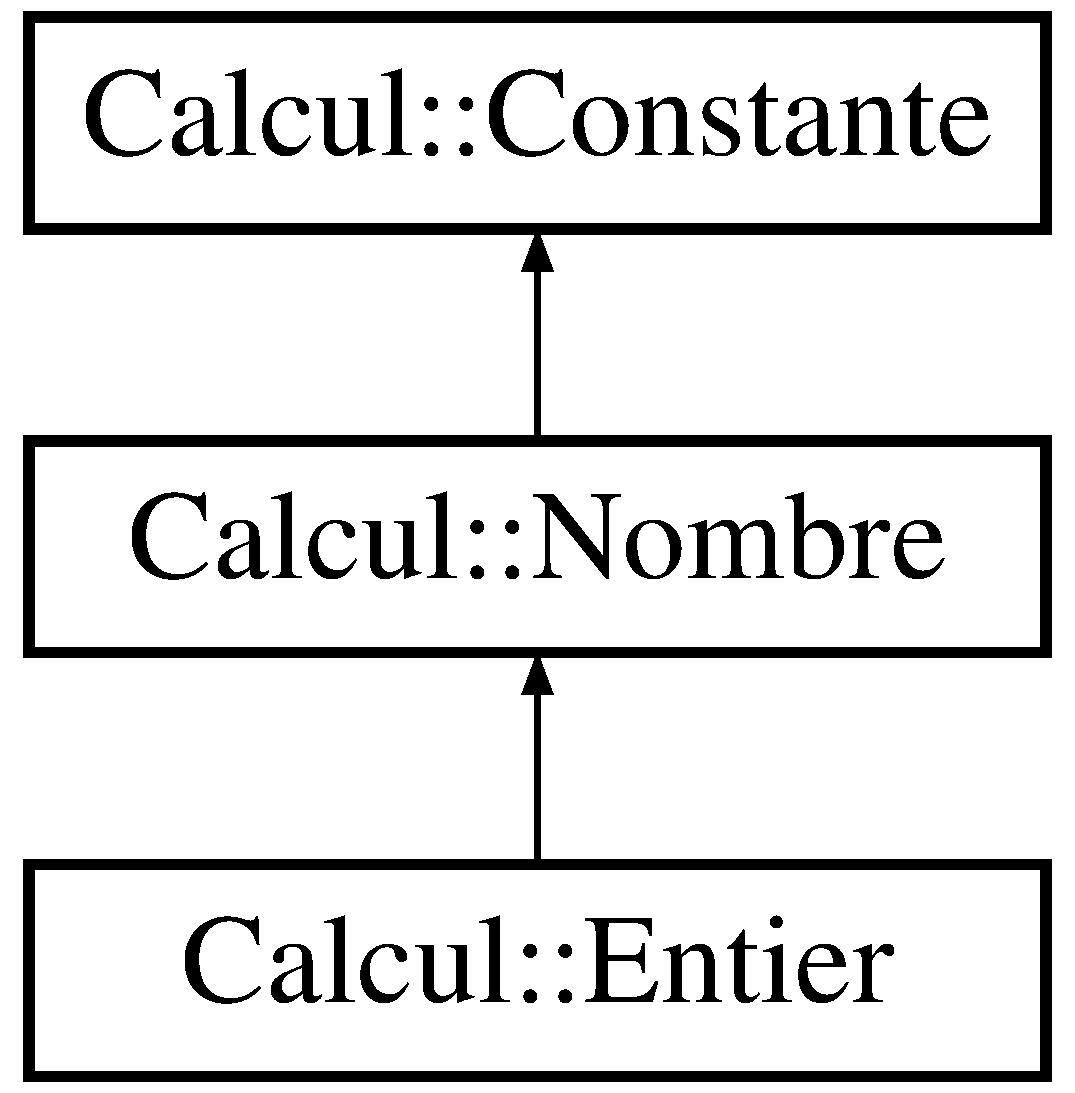
\includegraphics[height=3.000000cm]{class_calcul_1_1_entier}
\end{center}
\end{figure}
\subsection*{Public Member Functions}
\begin{DoxyCompactItemize}
\item 
\hypertarget{class_calcul_1_1_entier_aa95e3fe95acf3f49833246dea376e020}{{\bfseries Entier} (Q\-String e=\char`\"{}0\char`\"{})}\label{class_calcul_1_1_entier_aa95e3fe95acf3f49833246dea376e020}

\item 
\hypertarget{class_calcul_1_1_entier_afbaaaf29663668771b65630b394f5224}{{\bfseries Entier} (int e)}\label{class_calcul_1_1_entier_afbaaaf29663668771b65630b394f5224}

\item 
\hypertarget{class_calcul_1_1_entier_a5c76d9b068af9beaf3bc792d45020303}{{\bfseries Entier} (\hyperlink{class_calcul_1_1_entier}{Entier} $\ast$e)}\label{class_calcul_1_1_entier_a5c76d9b068af9beaf3bc792d45020303}

\item 
\hypertarget{class_calcul_1_1_entier_a2c99d3c3f8ec5346b94e3466b940cf99}{int {\bfseries Get\-Entier} () const }\label{class_calcul_1_1_entier_a2c99d3c3f8ec5346b94e3466b940cf99}

\item 
\hypertarget{class_calcul_1_1_entier_a7b917c5e0a8ae9278cf0ee0092ba608c}{double {\bfseries Get\-Reel} () const }\label{class_calcul_1_1_entier_a7b917c5e0a8ae9278cf0ee0092ba608c}

\item 
\hypertarget{class_calcul_1_1_entier_a3dd4de5f5c21961124d2a57613b7009d}{\hyperlink{class_calcul_1_1_reel}{Reel} {\bfseries to\-Reel} ()}\label{class_calcul_1_1_entier_a3dd4de5f5c21961124d2a57613b7009d}

\item 
\hypertarget{class_calcul_1_1_entier_a5797bcf92c69da8d07ce6f1c509a3dbe}{\hyperlink{class_calcul_1_1_rationnel}{Rationnel} {\bfseries to\-Rationnel} ()}\label{class_calcul_1_1_entier_a5797bcf92c69da8d07ce6f1c509a3dbe}

\item 
\hypertarget{class_calcul_1_1_entier_a7d0bcf436ce6517b8738f79eadda1f8a}{\hyperlink{class_calcul_1_1_complexe}{Complexe} {\bfseries to\-Complexe} ()}\label{class_calcul_1_1_entier_a7d0bcf436ce6517b8738f79eadda1f8a}

\item 
\hypertarget{class_calcul_1_1_entier_ae8e0b25ab85569d478cce96f02d31959}{const Q\-String {\bfseries Convert\-Chaine} () const }\label{class_calcul_1_1_entier_ae8e0b25ab85569d478cce96f02d31959}

\item 
\hypertarget{class_calcul_1_1_entier_a13aa8e43481bc82d84924fddc43b37d9}{\hyperlink{class_calcul_1_1_entier}{Entier} {\bfseries operator+} (\hyperlink{class_calcul_1_1_entier}{Entier} r1)}\label{class_calcul_1_1_entier_a13aa8e43481bc82d84924fddc43b37d9}

\item 
\hypertarget{class_calcul_1_1_entier_a831d41b5cfc26059bf2cc4455796f6e1}{\hyperlink{class_calcul_1_1_reel}{Reel} {\bfseries operator+} (\hyperlink{class_calcul_1_1_reel}{Reel} r1)}\label{class_calcul_1_1_entier_a831d41b5cfc26059bf2cc4455796f6e1}

\item 
\hypertarget{class_calcul_1_1_entier_a9430904a69b2e65ba3055d743466f2c2}{\hyperlink{class_calcul_1_1_rationnel}{Rationnel} {\bfseries operator+} (\hyperlink{class_calcul_1_1_rationnel}{Rationnel} r1)}\label{class_calcul_1_1_entier_a9430904a69b2e65ba3055d743466f2c2}

\item 
\hypertarget{class_calcul_1_1_entier_a49d7df865167f7a05113139511ec3476}{\hyperlink{class_calcul_1_1_nombre}{Nombre} $\ast$ {\bfseries operator+} (\hyperlink{class_calcul_1_1_nombre}{Nombre} $\ast$r1)}\label{class_calcul_1_1_entier_a49d7df865167f7a05113139511ec3476}

\item 
\hypertarget{class_calcul_1_1_entier_a8e3c581e835eccc9e62863934149a129}{\hyperlink{class_calcul_1_1_constante}{Constante} $\ast$ {\bfseries operator+} (\hyperlink{class_calcul_1_1_constante}{Constante} $\ast$r1)}\label{class_calcul_1_1_entier_a8e3c581e835eccc9e62863934149a129}

\item 
\hypertarget{class_calcul_1_1_entier_a79d8a8506c275b339d01663c2dfb67d8}{\hyperlink{class_calcul_1_1_entier}{Entier} {\bfseries operator-\/} (\hyperlink{class_calcul_1_1_entier}{Entier} r1)}\label{class_calcul_1_1_entier_a79d8a8506c275b339d01663c2dfb67d8}

\item 
\hypertarget{class_calcul_1_1_entier_a187a9ba0733ab36a3abf3e18a22647d6}{\hyperlink{class_calcul_1_1_entier}{Entier} {\bfseries operator-\/} ()}\label{class_calcul_1_1_entier_a187a9ba0733ab36a3abf3e18a22647d6}

\item 
\hypertarget{class_calcul_1_1_entier_a328b819a8caab0729cfa0da9faf4a4bc}{\hyperlink{class_calcul_1_1_reel}{Reel} {\bfseries operator-\/} (\hyperlink{class_calcul_1_1_reel}{Reel} r1)}\label{class_calcul_1_1_entier_a328b819a8caab0729cfa0da9faf4a4bc}

\item 
\hypertarget{class_calcul_1_1_entier_a449e8be1b0aaa580f7c0422037fa1a3b}{\hyperlink{class_calcul_1_1_rationnel}{Rationnel} {\bfseries operator-\/} (\hyperlink{class_calcul_1_1_rationnel}{Rationnel} r1)}\label{class_calcul_1_1_entier_a449e8be1b0aaa580f7c0422037fa1a3b}

\item 
\hypertarget{class_calcul_1_1_entier_a6308c4ec8d1e1b1e950c65f0ad6ebe43}{\hyperlink{class_calcul_1_1_nombre}{Nombre} $\ast$ {\bfseries operator-\/} (\hyperlink{class_calcul_1_1_nombre}{Nombre} $\ast$r1)}\label{class_calcul_1_1_entier_a6308c4ec8d1e1b1e950c65f0ad6ebe43}

\item 
\hypertarget{class_calcul_1_1_entier_a74ce097eac8e51fe551f39e6a59d1a42}{\hyperlink{class_calcul_1_1_constante}{Constante} $\ast$ {\bfseries operator-\/} (\hyperlink{class_calcul_1_1_constante}{Constante} $\ast$r1)}\label{class_calcul_1_1_entier_a74ce097eac8e51fe551f39e6a59d1a42}

\item 
\hypertarget{class_calcul_1_1_entier_ad1ca7e390b213f751e50a080476bd837}{\hyperlink{class_calcul_1_1_entier}{Entier} {\bfseries operator$\ast$} (\hyperlink{class_calcul_1_1_entier}{Entier} r1)}\label{class_calcul_1_1_entier_ad1ca7e390b213f751e50a080476bd837}

\item 
\hypertarget{class_calcul_1_1_entier_a35866eeafd779bb208e8e6738a6a8246}{\hyperlink{class_calcul_1_1_reel}{Reel} {\bfseries operator$\ast$} (\hyperlink{class_calcul_1_1_reel}{Reel} r1)}\label{class_calcul_1_1_entier_a35866eeafd779bb208e8e6738a6a8246}

\item 
\hypertarget{class_calcul_1_1_entier_aecca1f83490ea5ff205f5a6e0899cd46}{\hyperlink{class_calcul_1_1_rationnel}{Rationnel} {\bfseries operator$\ast$} (\hyperlink{class_calcul_1_1_rationnel}{Rationnel} r1)}\label{class_calcul_1_1_entier_aecca1f83490ea5ff205f5a6e0899cd46}

\item 
\hypertarget{class_calcul_1_1_entier_a0f92cec8dfd057a71ad995f0f08cea1c}{\hyperlink{class_calcul_1_1_nombre}{Nombre} $\ast$ {\bfseries operator$\ast$} (\hyperlink{class_calcul_1_1_nombre}{Nombre} $\ast$r1)}\label{class_calcul_1_1_entier_a0f92cec8dfd057a71ad995f0f08cea1c}

\item 
\hypertarget{class_calcul_1_1_entier_ae7a7907d1b6ca6861cda848a74724f72}{\hyperlink{class_calcul_1_1_constante}{Constante} $\ast$ {\bfseries operator$\ast$} (\hyperlink{class_calcul_1_1_constante}{Constante} $\ast$r1)}\label{class_calcul_1_1_entier_ae7a7907d1b6ca6861cda848a74724f72}

\item 
\hypertarget{class_calcul_1_1_entier_a58e327f828ca5ba2781ab7eeb42b658a}{\hyperlink{class_calcul_1_1_reel}{Reel} {\bfseries operator/} (\hyperlink{class_calcul_1_1_reel}{Reel} r1)}\label{class_calcul_1_1_entier_a58e327f828ca5ba2781ab7eeb42b658a}

\item 
\hypertarget{class_calcul_1_1_entier_af8cc637c5684a777cee5d2da989ce5b3}{\hyperlink{class_calcul_1_1_rationnel}{Rationnel} {\bfseries operator/} (\hyperlink{class_calcul_1_1_entier}{Entier} r1)}\label{class_calcul_1_1_entier_af8cc637c5684a777cee5d2da989ce5b3}

\item 
\hypertarget{class_calcul_1_1_entier_a2e48b86a6eee5dcdc0511928e621fb31}{\hyperlink{class_calcul_1_1_rationnel}{Rationnel} {\bfseries operator/} (\hyperlink{class_calcul_1_1_rationnel}{Rationnel} r1)}\label{class_calcul_1_1_entier_a2e48b86a6eee5dcdc0511928e621fb31}

\item 
\hypertarget{class_calcul_1_1_entier_add1e532abcbb17c847c6b81154eac4b2}{\hyperlink{class_calcul_1_1_nombre}{Nombre} $\ast$ {\bfseries operator/} (\hyperlink{class_calcul_1_1_nombre}{Nombre} $\ast$r1)}\label{class_calcul_1_1_entier_add1e532abcbb17c847c6b81154eac4b2}

\item 
\hypertarget{class_calcul_1_1_entier_aa7baff318fe0a94fbc3eef186977c159}{\hyperlink{class_calcul_1_1_constante}{Constante} $\ast$ {\bfseries operator/} (\hyperlink{class_calcul_1_1_constante}{Constante} $\ast$r1)}\label{class_calcul_1_1_entier_aa7baff318fe0a94fbc3eef186977c159}

\item 
\hypertarget{class_calcul_1_1_entier_a137cb0000f3fcbfe06cfffccd1dcc93e}{\hyperlink{class_calcul_1_1_reel}{Reel} {\bfseries puissance} (\hyperlink{class_calcul_1_1_reel}{Reel} r1)}\label{class_calcul_1_1_entier_a137cb0000f3fcbfe06cfffccd1dcc93e}

\item 
\hypertarget{class_calcul_1_1_entier_aeb7091d0e981d0fd3bbfa98703205446}{\hyperlink{class_calcul_1_1_rationnel}{Rationnel} {\bfseries puissance} (\hyperlink{class_calcul_1_1_entier}{Entier} r1)}\label{class_calcul_1_1_entier_aeb7091d0e981d0fd3bbfa98703205446}

\item 
\hypertarget{class_calcul_1_1_entier_a60354ee299f6429847f5a9f018285240}{\hyperlink{class_calcul_1_1_reel}{Reel} {\bfseries puissance} (\hyperlink{class_calcul_1_1_rationnel}{Rationnel} r1)}\label{class_calcul_1_1_entier_a60354ee299f6429847f5a9f018285240}

\item 
\hypertarget{class_calcul_1_1_entier_a72cabfa498578cd46f9a5f8dbf6fbdcb}{\hyperlink{class_calcul_1_1_constante}{Constante} $\ast$ {\bfseries puissance} (\hyperlink{class_calcul_1_1_constante}{Constante} $\ast$r1)}\label{class_calcul_1_1_entier_a72cabfa498578cd46f9a5f8dbf6fbdcb}

\item 
\hypertarget{class_calcul_1_1_entier_ac3a6010d95f511e0bb4c43441776a9af}{\hyperlink{class_calcul_1_1_reel}{Reel} {\bfseries sinus} ()}\label{class_calcul_1_1_entier_ac3a6010d95f511e0bb4c43441776a9af}

\item 
\hypertarget{class_calcul_1_1_entier_a9f224aeca4a1cde3ecd5b1b137c54aa2}{\hyperlink{class_calcul_1_1_reel}{Reel} {\bfseries cosinus} ()}\label{class_calcul_1_1_entier_a9f224aeca4a1cde3ecd5b1b137c54aa2}

\item 
\hypertarget{class_calcul_1_1_entier_a7b5d5008474daa89ab9a4ebdc70ff0c8}{\hyperlink{class_calcul_1_1_reel}{Reel} {\bfseries tangente} ()}\label{class_calcul_1_1_entier_a7b5d5008474daa89ab9a4ebdc70ff0c8}

\item 
\hypertarget{class_calcul_1_1_entier_ab93444ce2d4217f6aa6caa3244869e96}{\hyperlink{class_calcul_1_1_reel}{Reel} {\bfseries sinush} ()}\label{class_calcul_1_1_entier_ab93444ce2d4217f6aa6caa3244869e96}

\item 
\hypertarget{class_calcul_1_1_entier_a6cdbfb712f70bbad41a9435b25df23fc}{\hyperlink{class_calcul_1_1_reel}{Reel} {\bfseries cosinush} ()}\label{class_calcul_1_1_entier_a6cdbfb712f70bbad41a9435b25df23fc}

\item 
\hypertarget{class_calcul_1_1_entier_a6b75a28dee1bd10217b9a36051de8f8d}{\hyperlink{class_calcul_1_1_reel}{Reel} {\bfseries tangenteh} ()}\label{class_calcul_1_1_entier_a6b75a28dee1bd10217b9a36051de8f8d}

\item 
\hypertarget{class_calcul_1_1_entier_a79b0d7adfa75d5660f6a10361dc8092a}{\hyperlink{class_calcul_1_1_reel}{Reel} {\bfseries ln} ()}\label{class_calcul_1_1_entier_a79b0d7adfa75d5660f6a10361dc8092a}

\item 
\hypertarget{class_calcul_1_1_entier_a7c87b9015ff5e9f41f017bb106f01bea}{\hyperlink{class_calcul_1_1_reel}{Reel} {\bfseries logdix} ()}\label{class_calcul_1_1_entier_a7c87b9015ff5e9f41f017bb106f01bea}

\item 
\hypertarget{class_calcul_1_1_entier_ab3e28ed4b6259effa2998d179c59a023}{\hyperlink{class_calcul_1_1_rationnel}{Rationnel} {\bfseries inv} ()}\label{class_calcul_1_1_entier_ab3e28ed4b6259effa2998d179c59a023}

\item 
\hypertarget{class_calcul_1_1_entier_a05258eaa39ecc76509832fc84c4ada12}{\hyperlink{class_calcul_1_1_reel}{Reel} {\bfseries rsqr} ()}\label{class_calcul_1_1_entier_a05258eaa39ecc76509832fc84c4ada12}

\item 
\hypertarget{class_calcul_1_1_entier_accf5c68078b59f2ef3490195042d5b24}{\hyperlink{class_calcul_1_1_entier}{Entier} {\bfseries sqr} ()}\label{class_calcul_1_1_entier_accf5c68078b59f2ef3490195042d5b24}

\item 
\hypertarget{class_calcul_1_1_entier_a83c2833fe6841dcaa0c10beea1750a67}{\hyperlink{class_calcul_1_1_entier}{Entier} {\bfseries cube} ()}\label{class_calcul_1_1_entier_a83c2833fe6841dcaa0c10beea1750a67}

\item 
\hypertarget{class_calcul_1_1_entier_a16bb18c00fcb6a4c554c3eac3ff0939d}{\hyperlink{class_calcul_1_1_entier}{Entier} {\bfseries mod} (\hyperlink{class_calcul_1_1_entier}{Entier} e)}\label{class_calcul_1_1_entier_a16bb18c00fcb6a4c554c3eac3ff0939d}

\item 
\hypertarget{class_calcul_1_1_entier_a15488e68a0c47b0fa36baa2b3553bce9}{\hyperlink{class_calcul_1_1_entier}{Entier} {\bfseries fact} ()}\label{class_calcul_1_1_entier_a15488e68a0c47b0fa36baa2b3553bce9}

\end{DoxyCompactItemize}


The documentation for this class was generated from the following files\-:\begin{DoxyCompactItemize}
\item 
Constantes.\-h\item 
Entier.\-cpp\end{DoxyCompactItemize}

\hypertarget{class_calcul_1_1_expression}{\section{Référence de la classe Calcul\-:\-:Expression}
\label{class_calcul_1_1_expression}\index{Calcul\-::\-Expression@{Calcul\-::\-Expression}}
}


Classe qui permet d'implémenter une expression à l'aide d'un Q\-String.  




{\ttfamily \#include $<$Constantes.\-h$>$}

Graphe d'héritage de Calcul\-:\-:Expression\-:\begin{figure}[H]
\begin{center}
\leavevmode
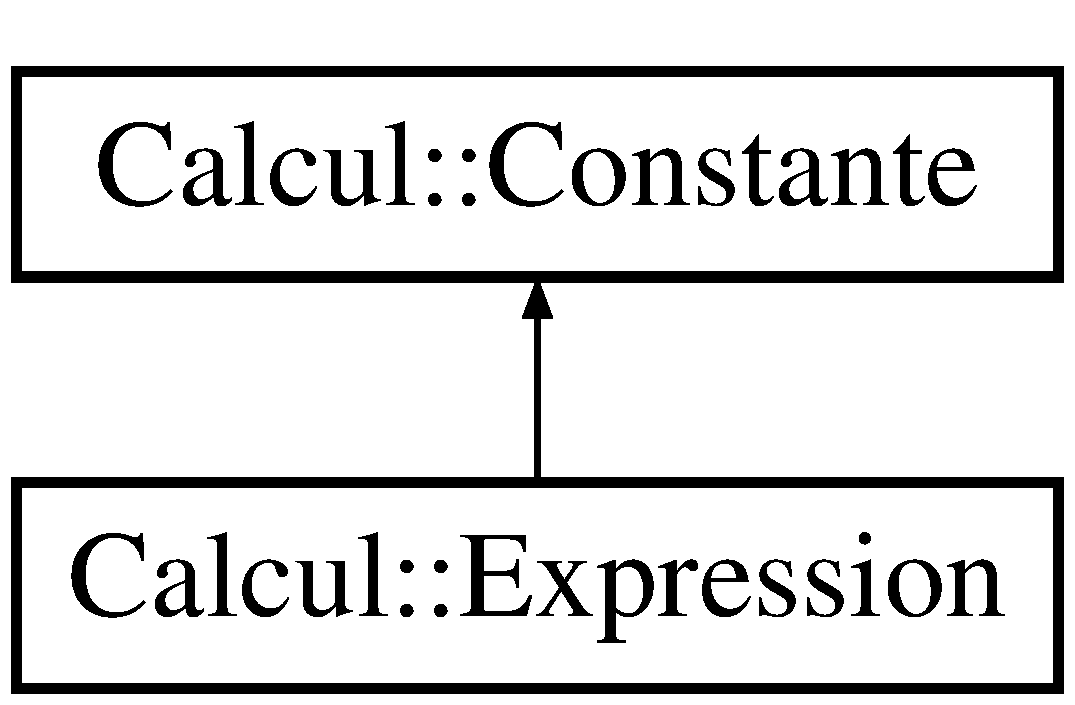
\includegraphics[height=2.000000cm]{class_calcul_1_1_expression}
\end{center}
\end{figure}
\subsection*{Fonctions membres publiques}
\begin{DoxyCompactItemize}
\item 
\hypertarget{class_calcul_1_1_expression_a756dc07653593481c4643d6a179d239b}{{\bfseries Expression} (Q\-String s)}\label{class_calcul_1_1_expression_a756dc07653593481c4643d6a179d239b}

\item 
\hypertarget{class_calcul_1_1_expression_a28a8ce64db734d8716f120b284a7e6df}{{\bfseries Expression} (\hyperlink{class_calcul_1_1_expression}{Expression} $\ast$e)}\label{class_calcul_1_1_expression_a28a8ce64db734d8716f120b284a7e6df}

\item 
const Q\-String \hyperlink{class_calcul_1_1_expression_a8bffbb504f9348cd69790c0fe23bf67d}{Convert\-Chaine} () const 
\begin{DoxyCompactList}\small\item\em Convert\-Chaine Méthode virtuelle qui convertit une \hyperlink{class_calcul_1_1_constante}{Constante} en une chaine de caractères. \end{DoxyCompactList}\item 
\hypertarget{class_calcul_1_1_expression_a240d6f19b3c3f3f5eebe3bddaa83f306}{bool {\bfseries is\-Null} ()}\label{class_calcul_1_1_expression_a240d6f19b3c3f3f5eebe3bddaa83f306}

\item 
\hypertarget{class_calcul_1_1_expression_af70b11f7b8fb7fc792df5628b932a117}{const Q\-String \hyperlink{class_calcul_1_1_expression_af70b11f7b8fb7fc792df5628b932a117}{Tronque} ()}\label{class_calcul_1_1_expression_af70b11f7b8fb7fc792df5628b932a117}

\begin{DoxyCompactList}\small\item\em Tronque retourne une \hyperlink{class_calcul_1_1_expression}{Expression}, sans ses quotes. \end{DoxyCompactList}\item 
void \hyperlink{class_calcul_1_1_expression_ac093ea5837a113f64be91e66b055b18b}{add\-Calcul} (Q\-String s)
\begin{DoxyCompactList}\small\item\em add\-Calcul \end{DoxyCompactList}\item 
void \hyperlink{class_calcul_1_1_expression_a0e762d07570ac388d0919a4c2053eecd}{calcul\-Add} (Q\-String s)
\begin{DoxyCompactList}\small\item\em calcul\-Add \end{DoxyCompactList}\end{DoxyCompactItemize}


\subsection{Description détaillée}
Classe qui permet d'implémenter une expression à l'aide d'un Q\-String. 

\subsection{Documentation des fonctions membres}
\hypertarget{class_calcul_1_1_expression_ac093ea5837a113f64be91e66b055b18b}{\index{Calcul\-::\-Expression@{Calcul\-::\-Expression}!add\-Calcul@{add\-Calcul}}
\index{add\-Calcul@{add\-Calcul}!Calcul::Expression@{Calcul\-::\-Expression}}
\subsubsection[{add\-Calcul}]{\setlength{\rightskip}{0pt plus 5cm}void Calcul\-::\-Expression\-::add\-Calcul (
\begin{DoxyParamCaption}
\item[{Q\-String}]{s}
\end{DoxyParamCaption}
)\hspace{0.3cm}{\ttfamily [inline]}}}\label{class_calcul_1_1_expression_ac093ea5837a113f64be91e66b055b18b}


add\-Calcul 

Ajoute un Q\-String a une expression, Q\-String ajouté à la fin 
\begin{DoxyParams}{Paramètres}
{\em Prend} & un Q\-String \\
\hline
\end{DoxyParams}
\hypertarget{class_calcul_1_1_expression_a0e762d07570ac388d0919a4c2053eecd}{\index{Calcul\-::\-Expression@{Calcul\-::\-Expression}!calcul\-Add@{calcul\-Add}}
\index{calcul\-Add@{calcul\-Add}!Calcul::Expression@{Calcul\-::\-Expression}}
\subsubsection[{calcul\-Add}]{\setlength{\rightskip}{0pt plus 5cm}void Calcul\-::\-Expression\-::calcul\-Add (
\begin{DoxyParamCaption}
\item[{Q\-String}]{s}
\end{DoxyParamCaption}
)\hspace{0.3cm}{\ttfamily [inline]}}}\label{class_calcul_1_1_expression_a0e762d07570ac388d0919a4c2053eecd}


calcul\-Add 

Ajoute un Q\-String a une expression, Q\-String ajouté au début 
\begin{DoxyParams}{Paramètres}
{\em Prend} & un Q\-String \\
\hline
\end{DoxyParams}
\hypertarget{class_calcul_1_1_expression_a8bffbb504f9348cd69790c0fe23bf67d}{\index{Calcul\-::\-Expression@{Calcul\-::\-Expression}!Convert\-Chaine@{Convert\-Chaine}}
\index{Convert\-Chaine@{Convert\-Chaine}!Calcul::Expression@{Calcul\-::\-Expression}}
\subsubsection[{Convert\-Chaine}]{\setlength{\rightskip}{0pt plus 5cm}const Q\-String Calcul\-::\-Expression\-::\-Convert\-Chaine (
\begin{DoxyParamCaption}
{}
\end{DoxyParamCaption}
) const\hspace{0.3cm}{\ttfamily [inline]}, {\ttfamily [virtual]}}}\label{class_calcul_1_1_expression_a8bffbb504f9348cd69790c0fe23bf67d}


Convert\-Chaine Méthode virtuelle qui convertit une \hyperlink{class_calcul_1_1_constante}{Constante} en une chaine de caractères. 

\begin{DoxyReturn}{Renvoie}
Retourne un const Q\-String 
\end{DoxyReturn}


Implémente \hyperlink{class_calcul_1_1_constante_a80fb461841b16e6d5d1339802b69858e}{Calcul\-::\-Constante}.



La documentation de cette classe a été générée à partir du fichier suivant \-:\begin{DoxyCompactItemize}
\item 
Projet\-\_\-\-L\-O21\-\_\-v3\-\_\-1/\hyperlink{_constantes_8h}{Constantes.\-h}\end{DoxyCompactItemize}

\hypertarget{class_fabrique_constante}{\section{Référence de la classe Fabrique\-Constante}
\label{class_fabrique_constante}\index{Fabrique\-Constante@{Fabrique\-Constante}}
}


Utilisation du design pattern factory pour créer des objets de type Constante.  




{\ttfamily \#include $<$Constante\-\_\-\-Factory.\-h$>$}

\subsection*{Fonctions membres publiques}
\begin{DoxyCompactItemize}
\item 
\hyperlink{class_calcul_1_1_constante}{Constante} $\ast$ \hyperlink{class_fabrique_constante_a7d192cf62b0c19f17d0ebdb8dac371ab}{get\-Constante} (Q\-String chaine)
\begin{DoxyCompactList}\small\item\em get\-Constante \end{DoxyCompactList}\item 
\hyperlink{class_calcul_1_1_constante}{Constante} $\ast$ \hyperlink{class_fabrique_constante_a05259a5b19903d8f1b640e45621d1fd4}{get\-Complexe} (Q\-String chaine)
\begin{DoxyCompactList}\small\item\em get\-Complexe \end{DoxyCompactList}\item 
\hyperlink{class_calcul_1_1_constante}{Constante} $\ast$ \hyperlink{class_fabrique_constante_a432cc65aa3d80402ea017963d5c06edf}{get\-Type} (\hyperlink{class_calcul_1_1_constante}{Constante} $\ast$a, int type)
\begin{DoxyCompactList}\small\item\em get\-Type \end{DoxyCompactList}\item 
\hyperlink{class_calcul_1_1_constante}{Constante} $\ast$ \hyperlink{class_fabrique_constante_aa1f4a720e896aaeabd85b0dc042c2ecf}{new\-Constante} (\hyperlink{class_calcul_1_1_constante}{Constante} $\ast$a)
\begin{DoxyCompactList}\small\item\em new\-Constante \end{DoxyCompactList}\end{DoxyCompactItemize}


\subsection{Description détaillée}
Utilisation du design pattern factory pour créer des objets de type Constante. 

\subsection{Documentation des fonctions membres}
\hypertarget{class_fabrique_constante_a05259a5b19903d8f1b640e45621d1fd4}{\index{Fabrique\-Constante@{Fabrique\-Constante}!get\-Complexe@{get\-Complexe}}
\index{get\-Complexe@{get\-Complexe}!FabriqueConstante@{Fabrique\-Constante}}
\subsubsection[{get\-Complexe}]{\setlength{\rightskip}{0pt plus 5cm}{\bf Constante} $\ast$ Fabrique\-Constante\-::get\-Complexe (
\begin{DoxyParamCaption}
\item[{Q\-String}]{chaine}
\end{DoxyParamCaption}
)}}\label{class_fabrique_constante_a05259a5b19903d8f1b640e45621d1fd4}


get\-Complexe 

Genère un Complexe à partir d'un Q\-String. Elle convertit tous les non Complexe en Complexe 
\begin{DoxyParams}{Paramètres}
{\em Q\-String} & contenant la Constante a générer \\
\hline
\end{DoxyParams}
\hypertarget{class_fabrique_constante_a7d192cf62b0c19f17d0ebdb8dac371ab}{\index{Fabrique\-Constante@{Fabrique\-Constante}!get\-Constante@{get\-Constante}}
\index{get\-Constante@{get\-Constante}!FabriqueConstante@{Fabrique\-Constante}}
\subsubsection[{get\-Constante}]{\setlength{\rightskip}{0pt plus 5cm}{\bf Constante} $\ast$ Fabrique\-Constante\-::get\-Constante (
\begin{DoxyParamCaption}
\item[{Q\-String}]{chaine}
\end{DoxyParamCaption}
)}}\label{class_fabrique_constante_a7d192cf62b0c19f17d0ebdb8dac371ab}


get\-Constante 

Genère une Constante à partir d'un Q\-String. 
\begin{DoxyParams}{Paramètres}
{\em Q\-String} & contenant la Constante a générer \\
\hline
\end{DoxyParams}
\hypertarget{class_fabrique_constante_a432cc65aa3d80402ea017963d5c06edf}{\index{Fabrique\-Constante@{Fabrique\-Constante}!get\-Type@{get\-Type}}
\index{get\-Type@{get\-Type}!FabriqueConstante@{Fabrique\-Constante}}
\subsubsection[{get\-Type}]{\setlength{\rightskip}{0pt plus 5cm}{\bf Constante} $\ast$ Fabrique\-Constante\-::get\-Type (
\begin{DoxyParamCaption}
\item[{{\bf Constante} $\ast$}]{a, }
\item[{int}]{type}
\end{DoxyParamCaption}
)}}\label{class_fabrique_constante_a432cc65aa3d80402ea017963d5c06edf}


get\-Type 

Genère une Constante à partir d'une Constante, en prenant compte d'un type de sortie (entier, réel, rationnel).  Constante$\ast$ à transformer  int contenant le type \hypertarget{class_fabrique_constante_aa1f4a720e896aaeabd85b0dc042c2ecf}{\index{Fabrique\-Constante@{Fabrique\-Constante}!new\-Constante@{new\-Constante}}
\index{new\-Constante@{new\-Constante}!FabriqueConstante@{Fabrique\-Constante}}
\subsubsection[{new\-Constante}]{\setlength{\rightskip}{0pt plus 5cm}{\bf Constante} $\ast$ Fabrique\-Constante\-::new\-Constante (
\begin{DoxyParamCaption}
\item[{{\bf Constante} $\ast$}]{a}
\end{DoxyParamCaption}
)}}\label{class_fabrique_constante_aa1f4a720e896aaeabd85b0dc042c2ecf}


new\-Constante 

Genère une Constante à partir d'un pointeur de Constante. Permet de dupliquer une Constante existante. 
\begin{DoxyParams}{Paramètres}
{\em Constante$\ast$} & à dupliquer \\
\hline
\end{DoxyParams}


La documentation de cette classe a été générée à partir des fichiers suivants \-:\begin{DoxyCompactItemize}
\item 
Projet\-\_\-\-L\-O21\-\_\-v3\-\_\-1/\hyperlink{_constante___factory_8h}{Constante\-\_\-\-Factory.\-h}\item 
Projet\-\_\-\-L\-O21\-\_\-v3\-\_\-1/\hyperlink{_constante___factory_8cpp}{Constante\-\_\-\-Factory.\-cpp}\end{DoxyCompactItemize}

\hypertarget{class_fabrique_nombre}{\section{Fabrique\-Nombre Class Reference}
\label{class_fabrique_nombre}\index{Fabrique\-Nombre@{Fabrique\-Nombre}}
}
\subsection*{Public Member Functions}
\begin{DoxyCompactItemize}
\item 
\hypertarget{class_fabrique_nombre_addd29295516c6899e5f7901595fdeddc}{\hyperlink{class_calcul_1_1_nombre}{Nombre} $\ast$ {\bfseries get\-Nombre} (Q\-String chaine)}\label{class_fabrique_nombre_addd29295516c6899e5f7901595fdeddc}

\item 
\hypertarget{class_fabrique_nombre_ab2284f484135ef2bc05f9d83fc37a76f}{\hyperlink{class_calcul_1_1_nombre}{Nombre} $\ast$ {\bfseries new\-Nombre} (\hyperlink{class_calcul_1_1_nombre}{Nombre} $\ast$a)}\label{class_fabrique_nombre_ab2284f484135ef2bc05f9d83fc37a76f}

\item 
\hypertarget{class_fabrique_nombre_a499d63c9f3da120b74a6b4a830f61aff}{\hyperlink{class_calcul_1_1_nombre}{Nombre} $\ast$ {\bfseries get\-Type} (\hyperlink{class_calcul_1_1_nombre}{Nombre} $\ast$a, int type)}\label{class_fabrique_nombre_a499d63c9f3da120b74a6b4a830f61aff}

\end{DoxyCompactItemize}


The documentation for this class was generated from the following files\-:\begin{DoxyCompactItemize}
\item 
Constante\-\_\-\-Factory.\-h\item 
Constante\-\_\-\-Factory.\-cpp\end{DoxyCompactItemize}

\hypertarget{class_main_window}{\section{Main\-Window Class Reference}
\label{class_main_window}\index{Main\-Window@{Main\-Window}}
}


Vue qui g�re l'affichage et communique avec \hyperlink{class_calculatrice_modele}{Calculatrice\-Modele} pour effectuer les calculs et rentrer les constantes.  




{\ttfamily \#include $<$mainwindow.\-h$>$}

\subsection*{Signals}
\begin{DoxyCompactItemize}
\item 
\hypertarget{class_main_window_ad223a3e425426fd76e3d40080096fc10}{void {\bfseries press\-Entrer\-N} (Q\-String s, bool complexe)}\label{class_main_window_ad223a3e425426fd76e3d40080096fc10}

\item 
\hypertarget{class_main_window_a7e430740aeaadb6d0d10514c979dab1a}{void {\bfseries fin\-Entree} ()}\label{class_main_window_a7e430740aeaadb6d0d10514c979dab1a}

\item 
\hypertarget{class_main_window_a95d2cfe9f1036d1dbbaad6d3f6504d1e}{void {\bfseries press\-Eval} ()}\label{class_main_window_a95d2cfe9f1036d1dbbaad6d3f6504d1e}

\item 
\hypertarget{class_main_window_aaf9db67eaf775db8b0bc1e066a844994}{void {\bfseries press\-Annuler} ()}\label{class_main_window_aaf9db67eaf775db8b0bc1e066a844994}

\item 
\hypertarget{class_main_window_a0e0214f53b83522b6fb4a513fdde0a56}{void {\bfseries press\-Retablir} ()}\label{class_main_window_a0e0214f53b83522b6fb4a513fdde0a56}

\item 
\hypertarget{class_main_window_ac966ffc012ed7b3df4615f4449281cec}{void {\bfseries complexe\-Vrai} ()}\label{class_main_window_ac966ffc012ed7b3df4615f4449281cec}

\item 
\hypertarget{class_main_window_aa20588e72485e9c17fcc81961296ebbf}{void {\bfseries complexe\-Faux} ()}\label{class_main_window_aa20588e72485e9c17fcc81961296ebbf}

\item 
\hypertarget{class_main_window_ad396facd02819cd66156a5229a02e6a7}{void {\bfseries press\-Add} (int type\-Nombre)}\label{class_main_window_ad396facd02819cd66156a5229a02e6a7}

\item 
\hypertarget{class_main_window_a4b349b6d265c94cb0327ea7204e89f38}{void {\bfseries press\-Sous} (int type\-Nombre)}\label{class_main_window_a4b349b6d265c94cb0327ea7204e89f38}

\item 
\hypertarget{class_main_window_a20be67f1bc010f1076d3ab1b0b7ca162}{void {\bfseries press\-Mult} (int type\-Nombre)}\label{class_main_window_a20be67f1bc010f1076d3ab1b0b7ca162}

\item 
\hypertarget{class_main_window_a97a8062c748d81bbc5462dd3cecb150d}{void {\bfseries press\-Div} (int type\-Nombre)}\label{class_main_window_a97a8062c748d81bbc5462dd3cecb150d}

\item 
\hypertarget{class_main_window_ac268a0536e2859f8622657aa8903f9dd}{void {\bfseries press\-Pow} (int type\-Nombre)}\label{class_main_window_ac268a0536e2859f8622657aa8903f9dd}

\item 
\hypertarget{class_main_window_a5f63c4865d583d26ef3315c8b14945c1}{void {\bfseries press\-Mod} ()}\label{class_main_window_a5f63c4865d583d26ef3315c8b14945c1}

\item 
\hypertarget{class_main_window_a1f4fe23c762eb48f8316945bbef42c62}{void {\bfseries press\-Fact} ()}\label{class_main_window_a1f4fe23c762eb48f8316945bbef42c62}

\item 
\hypertarget{class_main_window_af74e5eddba09f40bb96ad3052e5f4c85}{void {\bfseries press\-Sign} (int type\-Nombre)}\label{class_main_window_af74e5eddba09f40bb96ad3052e5f4c85}

\item 
\hypertarget{class_main_window_a225c94d2051035e146f27005e87bd3b9}{void {\bfseries press\-Sin} (bool degre)}\label{class_main_window_a225c94d2051035e146f27005e87bd3b9}

\item 
\hypertarget{class_main_window_aa7ee81851525510a160c872725c1cfe6}{void {\bfseries press\-Cos} (bool degre)}\label{class_main_window_aa7ee81851525510a160c872725c1cfe6}

\item 
\hypertarget{class_main_window_ae12de8cec7e19245ffd1e990f8edf865}{void {\bfseries press\-Tan} (bool degre)}\label{class_main_window_ae12de8cec7e19245ffd1e990f8edf865}

\item 
\hypertarget{class_main_window_a81ab0f96042e0b1e0708b6f756027d05}{void {\bfseries press\-Sinh} (bool degre)}\label{class_main_window_a81ab0f96042e0b1e0708b6f756027d05}

\item 
\hypertarget{class_main_window_ad48602c3caface8790147e4d742e1dc9}{void {\bfseries press\-Cosh} (bool degre)}\label{class_main_window_ad48602c3caface8790147e4d742e1dc9}

\item 
\hypertarget{class_main_window_a507253b1ad667b6c538fb3d8992bdc41}{void {\bfseries press\-Tanh} (bool degre)}\label{class_main_window_a507253b1ad667b6c538fb3d8992bdc41}

\item 
\hypertarget{class_main_window_a06cc8678a5a9af14cd036e041e76eef4}{void {\bfseries press\-Ln} ()}\label{class_main_window_a06cc8678a5a9af14cd036e041e76eef4}

\item 
\hypertarget{class_main_window_a8414825b291dc9a4965b8302b624c77d}{void {\bfseries press\-Log} ()}\label{class_main_window_a8414825b291dc9a4965b8302b624c77d}

\item 
\hypertarget{class_main_window_aad913fabae24bd877c0830f8d6cbfa1b}{void {\bfseries press\-Inv} (int type\-Nombre)}\label{class_main_window_aad913fabae24bd877c0830f8d6cbfa1b}

\item 
\hypertarget{class_main_window_a1cef6e994e88446eae146ec920588c36}{void {\bfseries press\-Sqrt} ()}\label{class_main_window_a1cef6e994e88446eae146ec920588c36}

\item 
\hypertarget{class_main_window_ad61a8b8a78c92453da2b55e4292e9d8c}{void {\bfseries press\-Sqr} (int type\-Nombre)}\label{class_main_window_ad61a8b8a78c92453da2b55e4292e9d8c}

\item 
\hypertarget{class_main_window_a3646c31c87248b33064cc83ad3b50f3c}{void {\bfseries press\-Cube} (int type\-Nombre)}\label{class_main_window_a3646c31c87248b33064cc83ad3b50f3c}

\item 
\hypertarget{class_main_window_a90f55dff8cd88ebb9ca51fbb45ff9572}{void {\bfseries press\-Swap} ()}\label{class_main_window_a90f55dff8cd88ebb9ca51fbb45ff9572}

\item 
\hypertarget{class_main_window_aad6db4cd90be3080ccfba45126f8314d}{void {\bfseries press\-Sum} (int type\-Nombre)}\label{class_main_window_aad6db4cd90be3080ccfba45126f8314d}

\item 
\hypertarget{class_main_window_af9af72599ae1edd0786d53b33548c02e}{void {\bfseries press\-Mean} (int type\-Nombre)}\label{class_main_window_af9af72599ae1edd0786d53b33548c02e}

\item 
\hypertarget{class_main_window_a7bfe416d75e010b19a746534be888500}{void {\bfseries press\-Clear} ()}\label{class_main_window_a7bfe416d75e010b19a746534be888500}

\item 
\hypertarget{class_main_window_a85c203aa98a11bff2fc1c04850c487f5}{void {\bfseries press\-Dup} ()}\label{class_main_window_a85c203aa98a11bff2fc1c04850c487f5}

\item 
\hypertarget{class_main_window_a7bf431a5544caa9134f78acaf4f5be96}{void {\bfseries press\-Drop} ()}\label{class_main_window_a7bf431a5544caa9134f78acaf4f5be96}

\end{DoxyCompactItemize}
\subsection*{Public Member Functions}
\begin{DoxyCompactItemize}
\item 
\hypertarget{class_main_window_a8b244be8b7b7db1b08de2a2acb9409db}{{\bfseries Main\-Window} (Q\-Widget $\ast$parent=0)}\label{class_main_window_a8b244be8b7b7db1b08de2a2acb9409db}

\end{DoxyCompactItemize}


\subsection{Detailed Description}
Vue qui g�re l'affichage et communique avec \hyperlink{class_calculatrice_modele}{Calculatrice\-Modele} pour effectuer les calculs et rentrer les constantes. 

{\itshape Fenetre\-Pile} permettra l'apparition d'une nouvelle fen�tre qui nous permettra la selection de la taille de la pile 

The documentation for this class was generated from the following files\-:\begin{DoxyCompactItemize}
\item 
mainwindow.\-h\item 
mainwindow.\-cpp\item 
Main\-Window\-Chiffres\-\_\-\-Operations.\-cpp\end{DoxyCompactItemize}

\hypertarget{class_calcul_1_1_nombre}{\section{Calcul\-:\-:Nombre Class Reference}
\label{class_calcul_1_1_nombre}\index{Calcul\-::\-Nombre@{Calcul\-::\-Nombre}}
}
Inheritance diagram for Calcul\-:\-:Nombre\-:\begin{figure}[H]
\begin{center}
\leavevmode
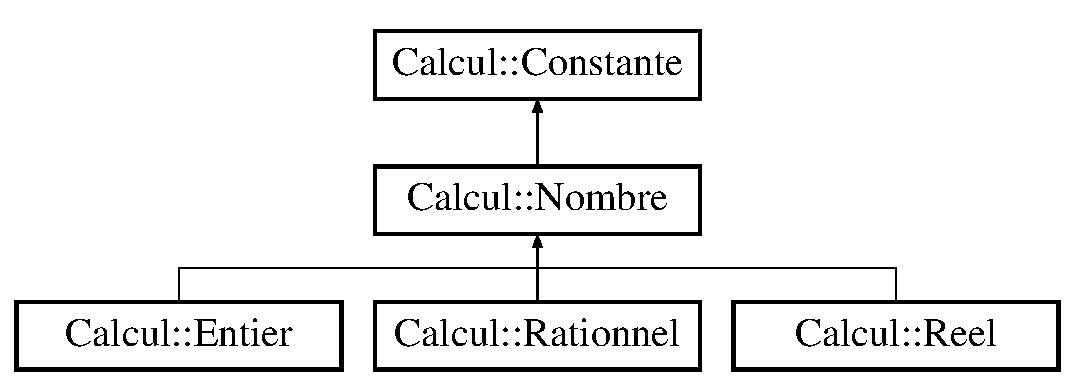
\includegraphics[height=3.000000cm]{class_calcul_1_1_nombre}
\end{center}
\end{figure}
\subsection*{Public Member Functions}
\begin{DoxyCompactItemize}
\item 
\hypertarget{class_calcul_1_1_nombre_a01b0c03ea3d7493e6d853768cce6f096}{virtual \hyperlink{class_calcul_1_1_complexe}{Complexe} {\bfseries to\-Complexe} ()=0}\label{class_calcul_1_1_nombre_a01b0c03ea3d7493e6d853768cce6f096}

\item 
\hypertarget{class_calcul_1_1_nombre_aa2a937e5d718f73f0edf25b702c11551}{virtual const Q\-String {\bfseries Convert\-Chaine} () const =0}\label{class_calcul_1_1_nombre_aa2a937e5d718f73f0edf25b702c11551}

\end{DoxyCompactItemize}


The documentation for this class was generated from the following file\-:\begin{DoxyCompactItemize}
\item 
Constantes.\-h\end{DoxyCompactItemize}

\hypertarget{class_calcul_1_1_rationnel}{\section{Référence de la classe Calcul\-:\-:Rationnel}
\label{class_calcul_1_1_rationnel}\index{Calcul\-::\-Rationnel@{Calcul\-::\-Rationnel}}
}


Classe qui permet d'implémenter un rationnel à l'aide de deux int.  




{\ttfamily \#include $<$Constantes.\-h$>$}

Graphe d'héritage de Calcul\-:\-:Rationnel\-:\begin{figure}[H]
\begin{center}
\leavevmode
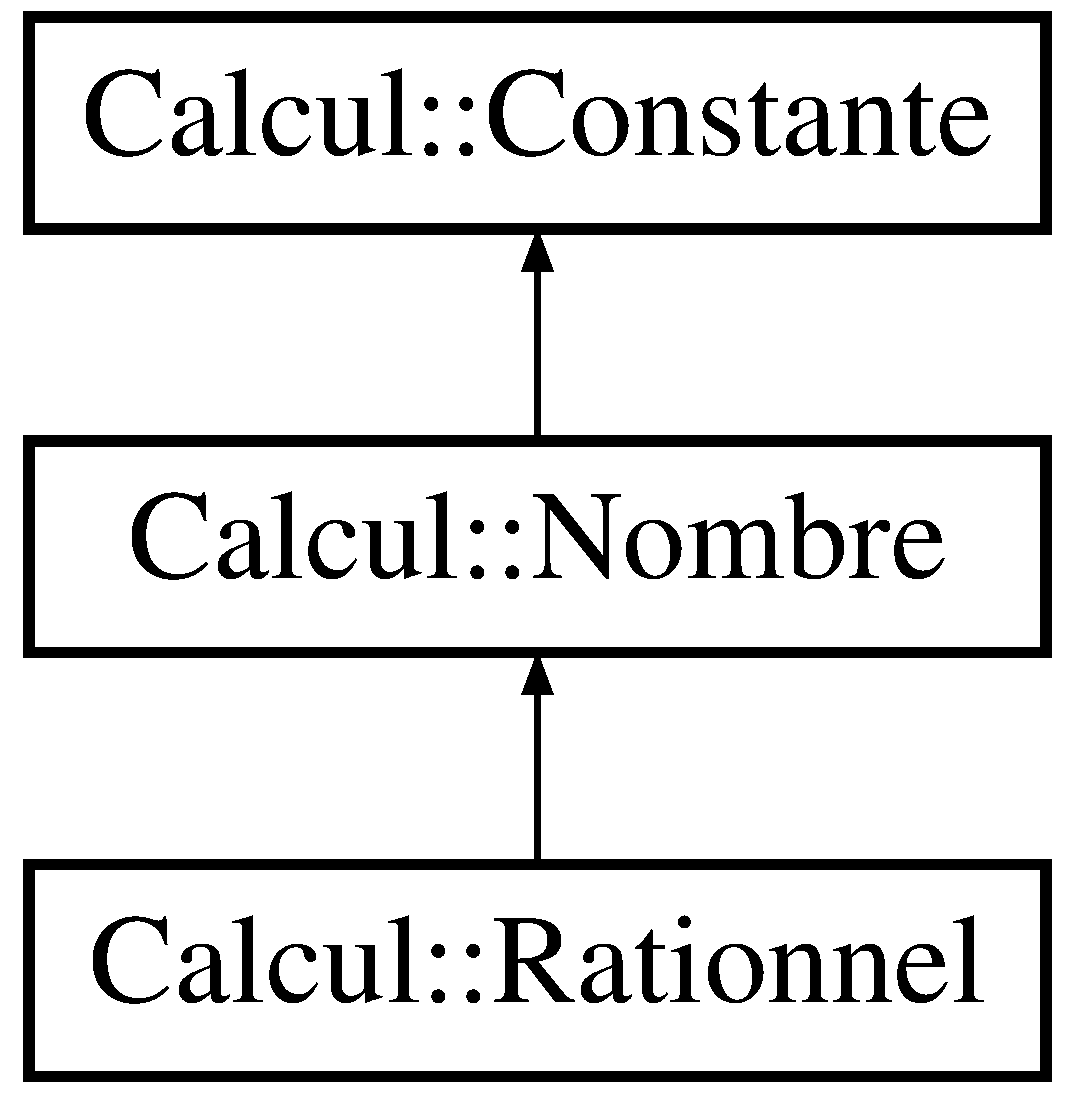
\includegraphics[height=3.000000cm]{class_calcul_1_1_rationnel}
\end{center}
\end{figure}
\subsection*{Fonctions membres publiques}
\begin{DoxyCompactItemize}
\item 
\hypertarget{class_calcul_1_1_rationnel_ac00a14054204cc5ea425c13ca6b68f8a}{{\bfseries Rationnel} (Q\-String s=\char`\"{}0/1\char`\"{})}\label{class_calcul_1_1_rationnel_ac00a14054204cc5ea425c13ca6b68f8a}

\item 
\hypertarget{class_calcul_1_1_rationnel_a9591906d6ed8040bf476afd8664cf29b}{{\bfseries Rationnel} (int n, int m=1)}\label{class_calcul_1_1_rationnel_a9591906d6ed8040bf476afd8664cf29b}

\item 
\hypertarget{class_calcul_1_1_rationnel_a1864157c6d295746a860363f2fe49572}{{\bfseries Rationnel} (\hyperlink{class_calcul_1_1_rationnel}{Rationnel} $\ast$r)}\label{class_calcul_1_1_rationnel_a1864157c6d295746a860363f2fe49572}

\item 
\hypertarget{class_calcul_1_1_rationnel_af6012e3151fddb2b27c50234a24ed30c}{void {\bfseries Set\-Num} (int n)}\label{class_calcul_1_1_rationnel_af6012e3151fddb2b27c50234a24ed30c}

\item 
\hypertarget{class_calcul_1_1_rationnel_ad184a895103274c732df6011a7d7e395}{void {\bfseries Set\-Den} (int n)}\label{class_calcul_1_1_rationnel_ad184a895103274c732df6011a7d7e395}

\item 
\hypertarget{class_calcul_1_1_rationnel_a7ec6d7a179032dd0008d216b7043a2df}{int {\bfseries Get\-Num} () const }\label{class_calcul_1_1_rationnel_a7ec6d7a179032dd0008d216b7043a2df}

\item 
\hypertarget{class_calcul_1_1_rationnel_abd1a6579f6fddfc99560fe3f106c3801}{int {\bfseries Get\-Den} () const }\label{class_calcul_1_1_rationnel_abd1a6579f6fddfc99560fe3f106c3801}

\item 
\hypertarget{class_calcul_1_1_rationnel_a96d32671b363d958578bb0c72f3ea20c}{double {\bfseries Get\-Rationnel} () const }\label{class_calcul_1_1_rationnel_a96d32671b363d958578bb0c72f3ea20c}

\item 
\hypertarget{class_calcul_1_1_rationnel_a235c633052410be850cadc514f8a906b}{void {\bfseries Simplification} ()}\label{class_calcul_1_1_rationnel_a235c633052410be850cadc514f8a906b}

\item 
\hypertarget{class_calcul_1_1_rationnel_afa1af66eebf420500eec16e3e8613227}{\hyperlink{class_calcul_1_1_entier}{Entier} {\bfseries to\-Entier} ()}\label{class_calcul_1_1_rationnel_afa1af66eebf420500eec16e3e8613227}

\item 
\hypertarget{class_calcul_1_1_rationnel_a29e6e8102f8484904723a053d334e90d}{\hyperlink{class_calcul_1_1_reel}{Reel} {\bfseries to\-Reel} ()}\label{class_calcul_1_1_rationnel_a29e6e8102f8484904723a053d334e90d}

\item 
\hyperlink{class_calcul_1_1_complexe}{Complexe} \hyperlink{class_calcul_1_1_rationnel_aad6bfa4160014c1ad603373a31383d76}{to\-Complexe} ()
\begin{DoxyCompactList}\small\item\em to\-Complexe \end{DoxyCompactList}\item 
const Q\-String \hyperlink{class_calcul_1_1_rationnel_acfec5903b8b8b5d2b80637a938966ce8}{Convert\-Chaine} () const 
\begin{DoxyCompactList}\small\item\em Convert\-Chaine Méthode virtuelle qui convertit une \hyperlink{class_calcul_1_1_constante}{Constante} en une chaine de caractères. \end{DoxyCompactList}\item 
\hypertarget{class_calcul_1_1_rationnel_a2cd8fe172adde56d15855af2aeb31259}{bool {\bfseries is\-Null} ()}\label{class_calcul_1_1_rationnel_a2cd8fe172adde56d15855af2aeb31259}

\item 
\hypertarget{class_calcul_1_1_rationnel_afbd51679a2eed2444effaee5a548e686}{bool {\bfseries is\-Positif} ()}\label{class_calcul_1_1_rationnel_afbd51679a2eed2444effaee5a548e686}

\item 
\hypertarget{class_calcul_1_1_rationnel_a32fcf45cb9ee316a613b862ff339bf07}{\hyperlink{class_calcul_1_1_rationnel}{Rationnel} {\bfseries operator+} (\hyperlink{class_calcul_1_1_rationnel}{Rationnel} r1)}\label{class_calcul_1_1_rationnel_a32fcf45cb9ee316a613b862ff339bf07}

\item 
\hypertarget{class_calcul_1_1_rationnel_ac6052754e4b2ad3af337f5272a348d6d}{\hyperlink{class_calcul_1_1_rationnel}{Rationnel} {\bfseries operator+} (\hyperlink{class_calcul_1_1_entier}{Entier} r1)}\label{class_calcul_1_1_rationnel_ac6052754e4b2ad3af337f5272a348d6d}

\item 
\hypertarget{class_calcul_1_1_rationnel_a2a8e787e497b145b1f463301639a9276}{\hyperlink{class_calcul_1_1_reel}{Reel} {\bfseries operator+} (\hyperlink{class_calcul_1_1_reel}{Reel} r1)}\label{class_calcul_1_1_rationnel_a2a8e787e497b145b1f463301639a9276}

\item 
\hypertarget{class_calcul_1_1_rationnel_ab921ad08242c9d4e813ae4c0c653c419}{\hyperlink{class_calcul_1_1_nombre}{Nombre} $\ast$ {\bfseries operator+} (\hyperlink{class_calcul_1_1_nombre}{Nombre} $\ast$r1)}\label{class_calcul_1_1_rationnel_ab921ad08242c9d4e813ae4c0c653c419}

\item 
\hypertarget{class_calcul_1_1_rationnel_a28bd8185e8550339b6a0c02eacf19f6a}{\hyperlink{class_calcul_1_1_constante}{Constante} $\ast$ {\bfseries operator+} (\hyperlink{class_calcul_1_1_constante}{Constante} $\ast$r1)}\label{class_calcul_1_1_rationnel_a28bd8185e8550339b6a0c02eacf19f6a}

\item 
\hypertarget{class_calcul_1_1_rationnel_a440c68e71f73c3cfa56d9962bc3d9a4e}{\hyperlink{class_calcul_1_1_rationnel}{Rationnel} {\bfseries operator-\/} (\hyperlink{class_calcul_1_1_rationnel}{Rationnel} r1)}\label{class_calcul_1_1_rationnel_a440c68e71f73c3cfa56d9962bc3d9a4e}

\item 
\hypertarget{class_calcul_1_1_rationnel_a673df26be184486eb82f41c4cfc95157}{\hyperlink{class_calcul_1_1_rationnel}{Rationnel} {\bfseries operator-\/} ()}\label{class_calcul_1_1_rationnel_a673df26be184486eb82f41c4cfc95157}

\item 
\hypertarget{class_calcul_1_1_rationnel_abb4e87e6a6f37e846ddc84bf45e86f5e}{\hyperlink{class_calcul_1_1_rationnel}{Rationnel} {\bfseries operator-\/} (\hyperlink{class_calcul_1_1_entier}{Entier} r1)}\label{class_calcul_1_1_rationnel_abb4e87e6a6f37e846ddc84bf45e86f5e}

\item 
\hypertarget{class_calcul_1_1_rationnel_a16d673d09ac7e8f180f5c5a0c7dc8a1a}{\hyperlink{class_calcul_1_1_reel}{Reel} {\bfseries operator-\/} (\hyperlink{class_calcul_1_1_reel}{Reel} r1)}\label{class_calcul_1_1_rationnel_a16d673d09ac7e8f180f5c5a0c7dc8a1a}

\item 
\hypertarget{class_calcul_1_1_rationnel_a7f00b197cea9a436270e4c2267eb8bda}{\hyperlink{class_calcul_1_1_nombre}{Nombre} $\ast$ {\bfseries operator-\/} (\hyperlink{class_calcul_1_1_nombre}{Nombre} $\ast$r1)}\label{class_calcul_1_1_rationnel_a7f00b197cea9a436270e4c2267eb8bda}

\item 
\hypertarget{class_calcul_1_1_rationnel_a2ded03b427948c223f6640c0956b1003}{\hyperlink{class_calcul_1_1_constante}{Constante} $\ast$ {\bfseries operator-\/} (\hyperlink{class_calcul_1_1_constante}{Constante} $\ast$r1)}\label{class_calcul_1_1_rationnel_a2ded03b427948c223f6640c0956b1003}

\item 
\hypertarget{class_calcul_1_1_rationnel_a9eb5a87ce8d78fe68f82daa64589b7d5}{\hyperlink{class_calcul_1_1_rationnel}{Rationnel} {\bfseries operator$\ast$} (\hyperlink{class_calcul_1_1_rationnel}{Rationnel} r1)}\label{class_calcul_1_1_rationnel_a9eb5a87ce8d78fe68f82daa64589b7d5}

\item 
\hypertarget{class_calcul_1_1_rationnel_af87f6c6ead1698fee973b20fd71307bf}{\hyperlink{class_calcul_1_1_rationnel}{Rationnel} {\bfseries operator$\ast$} (\hyperlink{class_calcul_1_1_entier}{Entier} r1)}\label{class_calcul_1_1_rationnel_af87f6c6ead1698fee973b20fd71307bf}

\item 
\hypertarget{class_calcul_1_1_rationnel_af71c6ab98b66231c6e46abb92d6ed797}{\hyperlink{class_calcul_1_1_reel}{Reel} {\bfseries operator$\ast$} (\hyperlink{class_calcul_1_1_reel}{Reel} r1)}\label{class_calcul_1_1_rationnel_af71c6ab98b66231c6e46abb92d6ed797}

\item 
\hypertarget{class_calcul_1_1_rationnel_a710f1b86e116ed059af45bc03711e774}{\hyperlink{class_calcul_1_1_nombre}{Nombre} $\ast$ {\bfseries operator$\ast$} (\hyperlink{class_calcul_1_1_nombre}{Nombre} $\ast$r1)}\label{class_calcul_1_1_rationnel_a710f1b86e116ed059af45bc03711e774}

\item 
\hypertarget{class_calcul_1_1_rationnel_ae1344b977d3c7c8fc2b1ed12fa7458b2}{\hyperlink{class_calcul_1_1_constante}{Constante} $\ast$ {\bfseries operator$\ast$} (\hyperlink{class_calcul_1_1_constante}{Constante} $\ast$r1)}\label{class_calcul_1_1_rationnel_ae1344b977d3c7c8fc2b1ed12fa7458b2}

\item 
\hypertarget{class_calcul_1_1_rationnel_a91327c85ae75d54ab389dfb442fa1490}{\hyperlink{class_calcul_1_1_rationnel}{Rationnel} {\bfseries operator/} (\hyperlink{class_calcul_1_1_rationnel}{Rationnel} r1)}\label{class_calcul_1_1_rationnel_a91327c85ae75d54ab389dfb442fa1490}

\item 
\hypertarget{class_calcul_1_1_rationnel_a4090e5817655c62283940fad4db6bdd2}{\hyperlink{class_calcul_1_1_rationnel}{Rationnel} {\bfseries operator/} (\hyperlink{class_calcul_1_1_entier}{Entier} r1)}\label{class_calcul_1_1_rationnel_a4090e5817655c62283940fad4db6bdd2}

\item 
\hypertarget{class_calcul_1_1_rationnel_a48e703bffb3015262d1ced7e80a963de}{\hyperlink{class_calcul_1_1_reel}{Reel} {\bfseries operator/} (\hyperlink{class_calcul_1_1_reel}{Reel} r1)}\label{class_calcul_1_1_rationnel_a48e703bffb3015262d1ced7e80a963de}

\item 
\hypertarget{class_calcul_1_1_rationnel_a9f24c10f89496da9e6cabe73795ce94f}{\hyperlink{class_calcul_1_1_nombre}{Nombre} $\ast$ {\bfseries operator/} (\hyperlink{class_calcul_1_1_nombre}{Nombre} $\ast$r1)}\label{class_calcul_1_1_rationnel_a9f24c10f89496da9e6cabe73795ce94f}

\item 
\hypertarget{class_calcul_1_1_rationnel_a910dff548e6a929af9f4e788e92cdf91}{\hyperlink{class_calcul_1_1_constante}{Constante} $\ast$ {\bfseries operator/} (\hyperlink{class_calcul_1_1_constante}{Constante} $\ast$r1)}\label{class_calcul_1_1_rationnel_a910dff548e6a929af9f4e788e92cdf91}

\item 
\hypertarget{class_calcul_1_1_rationnel_a1be47d3d22b8f9115b82081d1f419707}{\hyperlink{class_calcul_1_1_reel}{Reel} {\bfseries puissance} (\hyperlink{class_calcul_1_1_reel}{Reel} r1)}\label{class_calcul_1_1_rationnel_a1be47d3d22b8f9115b82081d1f419707}

\item 
\hypertarget{class_calcul_1_1_rationnel_ad799838a5d2fcb0a788732ae8748e2dd}{\hyperlink{class_calcul_1_1_rationnel}{Rationnel} {\bfseries puissance} (\hyperlink{class_calcul_1_1_entier}{Entier} r1)}\label{class_calcul_1_1_rationnel_ad799838a5d2fcb0a788732ae8748e2dd}

\item 
\hypertarget{class_calcul_1_1_rationnel_a03329a50dd162c16f6b769ccb1343fc2}{\hyperlink{class_calcul_1_1_reel}{Reel} {\bfseries puissance} (\hyperlink{class_calcul_1_1_rationnel}{Rationnel} r1)}\label{class_calcul_1_1_rationnel_a03329a50dd162c16f6b769ccb1343fc2}

\item 
\hypertarget{class_calcul_1_1_rationnel_afdbd441b846d8a0451f091b68e25968e}{\hyperlink{class_calcul_1_1_constante}{Constante} $\ast$ {\bfseries puissance} (\hyperlink{class_calcul_1_1_constante}{Constante} $\ast$r1)}\label{class_calcul_1_1_rationnel_afdbd441b846d8a0451f091b68e25968e}

\item 
\hypertarget{class_calcul_1_1_rationnel_a935c5d25b3e3b3e19f4b309cec412d26}{\hyperlink{class_calcul_1_1_reel}{Reel} {\bfseries sinus} ()}\label{class_calcul_1_1_rationnel_a935c5d25b3e3b3e19f4b309cec412d26}

\item 
\hypertarget{class_calcul_1_1_rationnel_ac1ecbfc18aec9fa8a88aeba133bd7417}{\hyperlink{class_calcul_1_1_reel}{Reel} {\bfseries cosinus} ()}\label{class_calcul_1_1_rationnel_ac1ecbfc18aec9fa8a88aeba133bd7417}

\item 
\hypertarget{class_calcul_1_1_rationnel_a658e15e265d7a69ac090b7dcb975b8b1}{\hyperlink{class_calcul_1_1_reel}{Reel} {\bfseries tangente} ()}\label{class_calcul_1_1_rationnel_a658e15e265d7a69ac090b7dcb975b8b1}

\item 
\hypertarget{class_calcul_1_1_rationnel_ae0363bd5486c42df55e603b635ac200c}{\hyperlink{class_calcul_1_1_reel}{Reel} {\bfseries sinush} ()}\label{class_calcul_1_1_rationnel_ae0363bd5486c42df55e603b635ac200c}

\item 
\hypertarget{class_calcul_1_1_rationnel_a90d87e81824f819b74946a1b999f79e6}{\hyperlink{class_calcul_1_1_reel}{Reel} {\bfseries cosinush} ()}\label{class_calcul_1_1_rationnel_a90d87e81824f819b74946a1b999f79e6}

\item 
\hypertarget{class_calcul_1_1_rationnel_a8d25f43222dcf910a36cecac200ece3e}{\hyperlink{class_calcul_1_1_reel}{Reel} {\bfseries tangenteh} ()}\label{class_calcul_1_1_rationnel_a8d25f43222dcf910a36cecac200ece3e}

\item 
\hypertarget{class_calcul_1_1_rationnel_ae8c11d80be50eacf53031e4638bf3025}{\hyperlink{class_calcul_1_1_reel}{Reel} $\ast$ {\bfseries ln} ()}\label{class_calcul_1_1_rationnel_ae8c11d80be50eacf53031e4638bf3025}

\item 
\hypertarget{class_calcul_1_1_rationnel_af469ec33aed69d09031c7104d8227229}{\hyperlink{class_calcul_1_1_reel}{Reel} $\ast$ {\bfseries logdix} ()}\label{class_calcul_1_1_rationnel_af469ec33aed69d09031c7104d8227229}

\item 
\hypertarget{class_calcul_1_1_rationnel_af532cbeab96518490c2aa521e3422cd4}{\hyperlink{class_calcul_1_1_rationnel}{Rationnel} $\ast$ {\bfseries inv} ()}\label{class_calcul_1_1_rationnel_af532cbeab96518490c2aa521e3422cd4}

\item 
\hypertarget{class_calcul_1_1_rationnel_a6f66761f74b75ecec7cd5963777fcbb0}{\hyperlink{class_calcul_1_1_reel}{Reel} $\ast$ {\bfseries rsqr} ()}\label{class_calcul_1_1_rationnel_a6f66761f74b75ecec7cd5963777fcbb0}

\item 
\hypertarget{class_calcul_1_1_rationnel_ab46637ec83548958a87fb7ded85c15f9}{\hyperlink{class_calcul_1_1_rationnel}{Rationnel} {\bfseries sqr} ()}\label{class_calcul_1_1_rationnel_ab46637ec83548958a87fb7ded85c15f9}

\item 
\hypertarget{class_calcul_1_1_rationnel_a663bd20d02eedbcd4bb8ab7eeab98086}{\hyperlink{class_calcul_1_1_rationnel}{Rationnel} {\bfseries cube} ()}\label{class_calcul_1_1_rationnel_a663bd20d02eedbcd4bb8ab7eeab98086}

\end{DoxyCompactItemize}
\subsection*{Attributs privés}
\begin{DoxyCompactItemize}
\item 
\hypertarget{class_calcul_1_1_rationnel_a8c56e1392d71b7bf0b3599a72d13210f}{int {\bfseries num}}\label{class_calcul_1_1_rationnel_a8c56e1392d71b7bf0b3599a72d13210f}

\item 
\hypertarget{class_calcul_1_1_rationnel_aa26f09c8eded353c64f0656e852760d1}{int {\bfseries den}}\label{class_calcul_1_1_rationnel_aa26f09c8eded353c64f0656e852760d1}

\end{DoxyCompactItemize}


\subsection{Description détaillée}
Classe qui permet d'implémenter un rationnel à l'aide de deux int. 

\subsection{Documentation des fonctions membres}
\hypertarget{class_calcul_1_1_rationnel_acfec5903b8b8b5d2b80637a938966ce8}{\index{Calcul\-::\-Rationnel@{Calcul\-::\-Rationnel}!Convert\-Chaine@{Convert\-Chaine}}
\index{Convert\-Chaine@{Convert\-Chaine}!Calcul::Rationnel@{Calcul\-::\-Rationnel}}
\subsubsection[{Convert\-Chaine}]{\setlength{\rightskip}{0pt plus 5cm}const Q\-String Calcul\-::\-Rationnel\-::\-Convert\-Chaine (
\begin{DoxyParamCaption}
{}
\end{DoxyParamCaption}
) const\hspace{0.3cm}{\ttfamily [inline]}, {\ttfamily [virtual]}}}\label{class_calcul_1_1_rationnel_acfec5903b8b8b5d2b80637a938966ce8}


Convert\-Chaine Méthode virtuelle qui convertit une \hyperlink{class_calcul_1_1_constante}{Constante} en une chaine de caractères. 

\begin{DoxyReturn}{Renvoie}
Retourne un const Q\-String 
\end{DoxyReturn}


Implémente \hyperlink{class_calcul_1_1_nombre_aa2a937e5d718f73f0edf25b702c11551}{Calcul\-::\-Nombre}.

\hypertarget{class_calcul_1_1_rationnel_aad6bfa4160014c1ad603373a31383d76}{\index{Calcul\-::\-Rationnel@{Calcul\-::\-Rationnel}!to\-Complexe@{to\-Complexe}}
\index{to\-Complexe@{to\-Complexe}!Calcul::Rationnel@{Calcul\-::\-Rationnel}}
\subsubsection[{to\-Complexe}]{\setlength{\rightskip}{0pt plus 5cm}{\bf Complexe} Calcul\-::\-Rationnel\-::to\-Complexe (
\begin{DoxyParamCaption}
{}
\end{DoxyParamCaption}
)\hspace{0.3cm}{\ttfamily [inline]}, {\ttfamily [virtual]}}}\label{class_calcul_1_1_rationnel_aad6bfa4160014c1ad603373a31383d76}


to\-Complexe 

Méthode virtuelle qui convertit un \hyperlink{class_calcul_1_1_nombre}{Nombre} en un \hyperlink{class_calcul_1_1_complexe}{Complexe} \begin{DoxyReturn}{Renvoie}
Retourne un complexe 
\end{DoxyReturn}


Implémente \hyperlink{class_calcul_1_1_nombre_a01b0c03ea3d7493e6d853768cce6f096}{Calcul\-::\-Nombre}.



La documentation de cette classe a été générée à partir des fichiers suivants \-:\begin{DoxyCompactItemize}
\item 
Projet\-\_\-\-L\-O21\-\_\-v3\-\_\-1/\hyperlink{_constantes_8h}{Constantes.\-h}\item 
Projet\-\_\-\-L\-O21\-\_\-v3\-\_\-1/\hyperlink{_rationnel_8cpp}{Rationnel.\-cpp}\end{DoxyCompactItemize}

\hypertarget{class_calcul_1_1_reel}{\section{Référence de la classe Calcul\-:\-:Reel}
\label{class_calcul_1_1_reel}\index{Calcul\-::\-Reel@{Calcul\-::\-Reel}}
}


Classe qui permet d'implémenter un réel à l'aide d'un double.  




{\ttfamily \#include $<$Constantes.\-h$>$}

Graphe d'héritage de Calcul\-:\-:Reel\-:\begin{figure}[H]
\begin{center}
\leavevmode
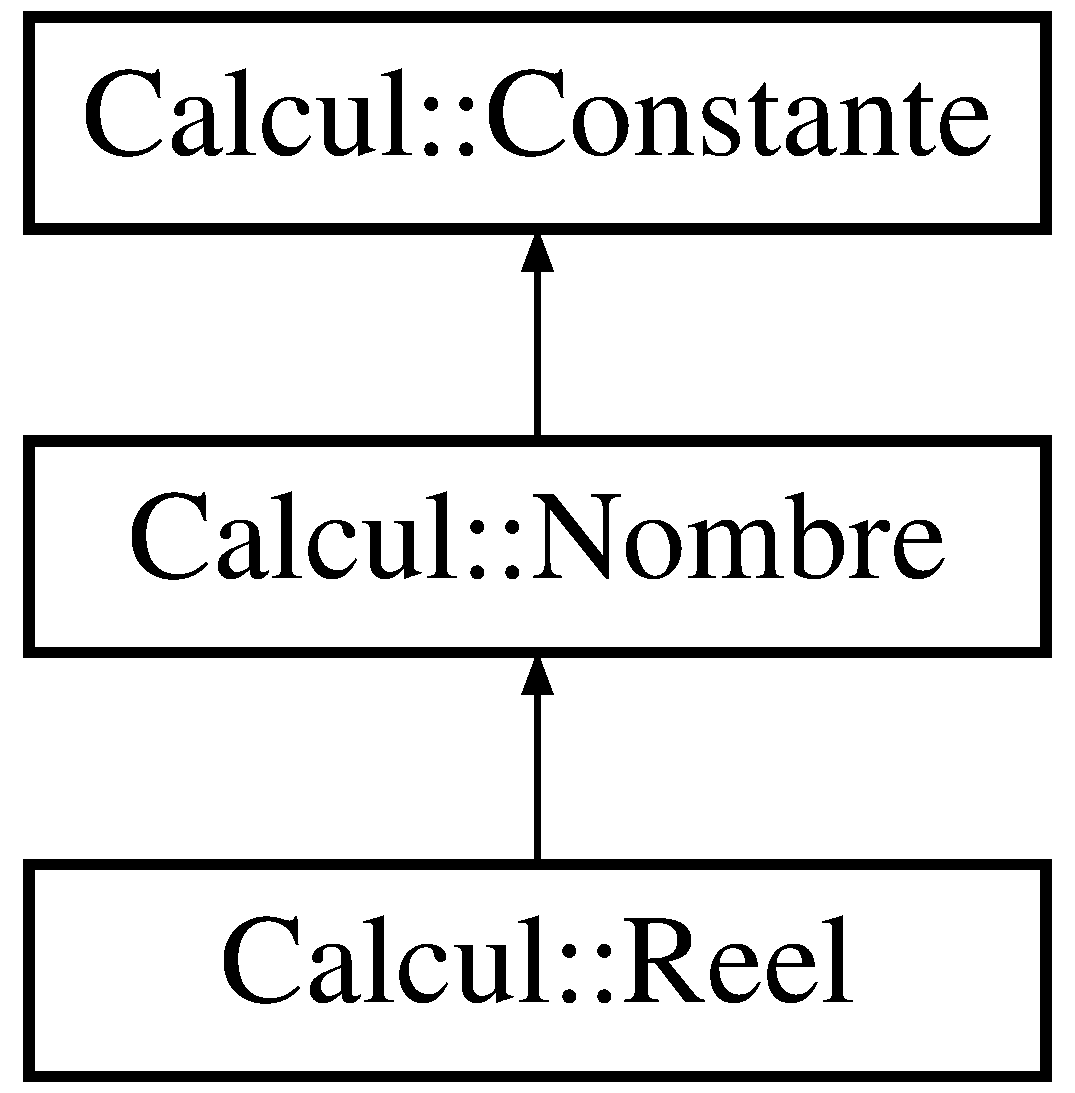
\includegraphics[height=3.000000cm]{class_calcul_1_1_reel}
\end{center}
\end{figure}
\subsection*{Fonctions membres publiques}
\begin{DoxyCompactItemize}
\item 
\hypertarget{class_calcul_1_1_reel_ae0b25df32769db7d5108c181b64657c2}{{\bfseries Reel} (Q\-String r=\char`\"{}0\char`\"{})}\label{class_calcul_1_1_reel_ae0b25df32769db7d5108c181b64657c2}

\item 
\hypertarget{class_calcul_1_1_reel_a19d0ce325d4a7a3b9a299b792702168a}{{\bfseries Reel} (double r)}\label{class_calcul_1_1_reel_a19d0ce325d4a7a3b9a299b792702168a}

\item 
\hypertarget{class_calcul_1_1_reel_a6b1310b24cd92b2d59a646cadc29f576}{{\bfseries Reel} (\hyperlink{class_calcul_1_1_reel}{Reel} $\ast$r)}\label{class_calcul_1_1_reel_a6b1310b24cd92b2d59a646cadc29f576}

\item 
\hypertarget{class_calcul_1_1_reel_a75a6a4a791f47a05c38b92244f6cf5a0}{double {\bfseries Get\-Reel} () const }\label{class_calcul_1_1_reel_a75a6a4a791f47a05c38b92244f6cf5a0}

\item 
\hypertarget{class_calcul_1_1_reel_a6660d6f839cf55825042f458a0ec7e54}{int {\bfseries Get\-Entier} () const }\label{class_calcul_1_1_reel_a6660d6f839cf55825042f458a0ec7e54}

\item 
\hypertarget{class_calcul_1_1_reel_ae334416316678b356875791e125ba14a}{\hyperlink{class_calcul_1_1_entier}{Entier} {\bfseries to\-Entier} ()}\label{class_calcul_1_1_reel_ae334416316678b356875791e125ba14a}

\item 
\hypertarget{class_calcul_1_1_reel_ae21a0235c35a7fbb87c7c36108d861b9}{\hyperlink{class_calcul_1_1_rationnel}{Rationnel} {\bfseries to\-Rationnel} ()}\label{class_calcul_1_1_reel_ae21a0235c35a7fbb87c7c36108d861b9}

\item 
\hyperlink{class_calcul_1_1_complexe}{Complexe} \hyperlink{class_calcul_1_1_reel_a222b9929b24dfee2928191055f1d03fa}{to\-Complexe} ()
\begin{DoxyCompactList}\small\item\em to\-Complexe \end{DoxyCompactList}\item 
const Q\-String \hyperlink{class_calcul_1_1_reel_a92c0a269edf334bba71b08ef0e9e27e8}{Convert\-Chaine} () const 
\begin{DoxyCompactList}\small\item\em Convert\-Chaine Méthode virtuelle qui convertit une \hyperlink{class_calcul_1_1_constante}{Constante} en une chaine de caractères. \end{DoxyCompactList}\item 
\hypertarget{class_calcul_1_1_reel_a892118585b915fb12426c3d636166be2}{bool {\bfseries is\-Null} ()}\label{class_calcul_1_1_reel_a892118585b915fb12426c3d636166be2}

\item 
\hypertarget{class_calcul_1_1_reel_a2476f8f9eaa5f34b76cef8b3197b2809}{bool {\bfseries is\-Positif} ()}\label{class_calcul_1_1_reel_a2476f8f9eaa5f34b76cef8b3197b2809}

\item 
\hypertarget{class_calcul_1_1_reel_a157b1e83c3807655d29289a1c72850a0}{\hyperlink{class_calcul_1_1_reel}{Reel} {\bfseries operator=} (\hyperlink{class_calcul_1_1_reel}{Reel} r1)}\label{class_calcul_1_1_reel_a157b1e83c3807655d29289a1c72850a0}

\item 
\hypertarget{class_calcul_1_1_reel_af9a5a6133c065863d2b2265253c3cc1c}{\hyperlink{class_calcul_1_1_reel}{Reel} {\bfseries operator+} (\hyperlink{class_calcul_1_1_reel}{Reel} r1)}\label{class_calcul_1_1_reel_af9a5a6133c065863d2b2265253c3cc1c}

\item 
\hypertarget{class_calcul_1_1_reel_a186d48551e5f909001a9553fadd2af36}{\hyperlink{class_calcul_1_1_reel}{Reel} {\bfseries operator+} (\hyperlink{class_calcul_1_1_entier}{Entier} r1)}\label{class_calcul_1_1_reel_a186d48551e5f909001a9553fadd2af36}

\item 
\hypertarget{class_calcul_1_1_reel_ae82fd9fd0ee3fcfc38920dd1b8edb35a}{\hyperlink{class_calcul_1_1_reel}{Reel} {\bfseries operator+} (\hyperlink{class_calcul_1_1_rationnel}{Rationnel} r1)}\label{class_calcul_1_1_reel_ae82fd9fd0ee3fcfc38920dd1b8edb35a}

\item 
\hypertarget{class_calcul_1_1_reel_a70c39fb22fa228e3ce2d1c42e239901c}{\hyperlink{class_calcul_1_1_nombre}{Nombre} $\ast$ {\bfseries operator+} (\hyperlink{class_calcul_1_1_nombre}{Nombre} $\ast$r1)}\label{class_calcul_1_1_reel_a70c39fb22fa228e3ce2d1c42e239901c}

\item 
\hypertarget{class_calcul_1_1_reel_a3188434518acd6fa8c9715f01389eadc}{\hyperlink{class_calcul_1_1_constante}{Constante} $\ast$ {\bfseries operator+} (\hyperlink{class_calcul_1_1_constante}{Constante} $\ast$r1)}\label{class_calcul_1_1_reel_a3188434518acd6fa8c9715f01389eadc}

\item 
\hypertarget{class_calcul_1_1_reel_af193c3b17e79a281ffa137060e8e6687}{\hyperlink{class_calcul_1_1_reel}{Reel} {\bfseries operator-\/} (\hyperlink{class_calcul_1_1_reel}{Reel} r1)}\label{class_calcul_1_1_reel_af193c3b17e79a281ffa137060e8e6687}

\item 
\hypertarget{class_calcul_1_1_reel_adfa38490921599d6b59bd293d3d4d8b2}{\hyperlink{class_calcul_1_1_reel}{Reel} {\bfseries operator-\/} ()}\label{class_calcul_1_1_reel_adfa38490921599d6b59bd293d3d4d8b2}

\item 
\hypertarget{class_calcul_1_1_reel_a804de5916ceaf36afb821a72839ffa96}{\hyperlink{class_calcul_1_1_reel}{Reel} {\bfseries operator-\/} (\hyperlink{class_calcul_1_1_entier}{Entier} r1)}\label{class_calcul_1_1_reel_a804de5916ceaf36afb821a72839ffa96}

\item 
\hypertarget{class_calcul_1_1_reel_a2aaabcf3c1b9afea62a757cd42fefc32}{\hyperlink{class_calcul_1_1_reel}{Reel} {\bfseries operator-\/} (\hyperlink{class_calcul_1_1_rationnel}{Rationnel} r1)}\label{class_calcul_1_1_reel_a2aaabcf3c1b9afea62a757cd42fefc32}

\item 
\hypertarget{class_calcul_1_1_reel_a68ce950fa5f597e346e1333d9cf341bd}{\hyperlink{class_calcul_1_1_nombre}{Nombre} $\ast$ {\bfseries operator-\/} (\hyperlink{class_calcul_1_1_nombre}{Nombre} $\ast$r1)}\label{class_calcul_1_1_reel_a68ce950fa5f597e346e1333d9cf341bd}

\item 
\hypertarget{class_calcul_1_1_reel_aeae8d7a5beb68d91daa895a485567da4}{\hyperlink{class_calcul_1_1_constante}{Constante} $\ast$ {\bfseries operator-\/} (\hyperlink{class_calcul_1_1_constante}{Constante} $\ast$r1)}\label{class_calcul_1_1_reel_aeae8d7a5beb68d91daa895a485567da4}

\item 
\hypertarget{class_calcul_1_1_reel_a8860ea9e054fcce2680da4275ae1823c}{\hyperlink{class_calcul_1_1_reel}{Reel} {\bfseries operator$\ast$} (\hyperlink{class_calcul_1_1_reel}{Reel} r1)}\label{class_calcul_1_1_reel_a8860ea9e054fcce2680da4275ae1823c}

\item 
\hypertarget{class_calcul_1_1_reel_a6b3d287264cb02e8d21c57b557a28eca}{\hyperlink{class_calcul_1_1_reel}{Reel} {\bfseries operator$\ast$} (\hyperlink{class_calcul_1_1_entier}{Entier} r1)}\label{class_calcul_1_1_reel_a6b3d287264cb02e8d21c57b557a28eca}

\item 
\hypertarget{class_calcul_1_1_reel_a67cf90af62fd20f86edb2f37e3686842}{\hyperlink{class_calcul_1_1_reel}{Reel} {\bfseries operator$\ast$} (\hyperlink{class_calcul_1_1_rationnel}{Rationnel} r1)}\label{class_calcul_1_1_reel_a67cf90af62fd20f86edb2f37e3686842}

\item 
\hypertarget{class_calcul_1_1_reel_a216ec2c031c1c8ad3f35763d288d1a4b}{\hyperlink{class_calcul_1_1_nombre}{Nombre} $\ast$ {\bfseries operator$\ast$} (\hyperlink{class_calcul_1_1_nombre}{Nombre} $\ast$r1)}\label{class_calcul_1_1_reel_a216ec2c031c1c8ad3f35763d288d1a4b}

\item 
\hypertarget{class_calcul_1_1_reel_afd4ca6b0c20fa732add38a59ac9ba870}{\hyperlink{class_calcul_1_1_constante}{Constante} $\ast$ {\bfseries operator$\ast$} (\hyperlink{class_calcul_1_1_constante}{Constante} $\ast$r1)}\label{class_calcul_1_1_reel_afd4ca6b0c20fa732add38a59ac9ba870}

\item 
\hypertarget{class_calcul_1_1_reel_a06a171e324dc40179bf05a37b251f3d6}{\hyperlink{class_calcul_1_1_reel}{Reel} {\bfseries operator/} (\hyperlink{class_calcul_1_1_reel}{Reel} r1)}\label{class_calcul_1_1_reel_a06a171e324dc40179bf05a37b251f3d6}

\item 
\hypertarget{class_calcul_1_1_reel_a8f51ae3ac33086e3e52e2d786c31a986}{\hyperlink{class_calcul_1_1_reel}{Reel} {\bfseries operator/} (\hyperlink{class_calcul_1_1_entier}{Entier} r1)}\label{class_calcul_1_1_reel_a8f51ae3ac33086e3e52e2d786c31a986}

\item 
\hypertarget{class_calcul_1_1_reel_a628dc4f82680abc641ee6af63681f81b}{\hyperlink{class_calcul_1_1_reel}{Reel} {\bfseries operator/} (\hyperlink{class_calcul_1_1_rationnel}{Rationnel} r1)}\label{class_calcul_1_1_reel_a628dc4f82680abc641ee6af63681f81b}

\item 
\hypertarget{class_calcul_1_1_reel_ae4a8fdaa5ee5e626b80936d2aa80fdf7}{\hyperlink{class_calcul_1_1_nombre}{Nombre} $\ast$ {\bfseries operator/} (\hyperlink{class_calcul_1_1_nombre}{Nombre} $\ast$r1)}\label{class_calcul_1_1_reel_ae4a8fdaa5ee5e626b80936d2aa80fdf7}

\item 
\hypertarget{class_calcul_1_1_reel_aa8ca5669752623a91c02387ac55a4a51}{\hyperlink{class_calcul_1_1_constante}{Constante} $\ast$ {\bfseries operator/} (\hyperlink{class_calcul_1_1_constante}{Constante} $\ast$r1)}\label{class_calcul_1_1_reel_aa8ca5669752623a91c02387ac55a4a51}

\item 
\hypertarget{class_calcul_1_1_reel_a40f9b7e8fed1f0ce48bd1c2856e93d77}{\hyperlink{class_calcul_1_1_reel}{Reel} {\bfseries puissance} (\hyperlink{class_calcul_1_1_reel}{Reel} r1)}\label{class_calcul_1_1_reel_a40f9b7e8fed1f0ce48bd1c2856e93d77}

\item 
\hypertarget{class_calcul_1_1_reel_af73aaf802976ef0c764329f823294a6c}{\hyperlink{class_calcul_1_1_reel}{Reel} {\bfseries puissance} (\hyperlink{class_calcul_1_1_entier}{Entier} r1)}\label{class_calcul_1_1_reel_af73aaf802976ef0c764329f823294a6c}

\item 
\hypertarget{class_calcul_1_1_reel_a622d831d687146689e364a764231e7f8}{\hyperlink{class_calcul_1_1_reel}{Reel} {\bfseries puissance} (\hyperlink{class_calcul_1_1_rationnel}{Rationnel} r1)}\label{class_calcul_1_1_reel_a622d831d687146689e364a764231e7f8}

\item 
\hypertarget{class_calcul_1_1_reel_a095095f9dc094d5633a57fe99a135614}{\hyperlink{class_calcul_1_1_constante}{Constante} $\ast$ {\bfseries puissance} (\hyperlink{class_calcul_1_1_constante}{Constante} $\ast$r1)}\label{class_calcul_1_1_reel_a095095f9dc094d5633a57fe99a135614}

\item 
\hypertarget{class_calcul_1_1_reel_a8e9b77be10a316dff79468ac9ed871f1}{\hyperlink{class_calcul_1_1_reel}{Reel} {\bfseries sinus} ()}\label{class_calcul_1_1_reel_a8e9b77be10a316dff79468ac9ed871f1}

\item 
\hypertarget{class_calcul_1_1_reel_ab069346c660bce5f6493445e3758ab51}{\hyperlink{class_calcul_1_1_reel}{Reel} {\bfseries cosinus} ()}\label{class_calcul_1_1_reel_ab069346c660bce5f6493445e3758ab51}

\item 
\hypertarget{class_calcul_1_1_reel_a1ca49402444ad59a968a26ef9328d89f}{\hyperlink{class_calcul_1_1_reel}{Reel} {\bfseries tangente} ()}\label{class_calcul_1_1_reel_a1ca49402444ad59a968a26ef9328d89f}

\item 
\hypertarget{class_calcul_1_1_reel_acc463533b4491b1ea474f0dd997c5d9d}{\hyperlink{class_calcul_1_1_reel}{Reel} {\bfseries sinush} ()}\label{class_calcul_1_1_reel_acc463533b4491b1ea474f0dd997c5d9d}

\item 
\hypertarget{class_calcul_1_1_reel_ab3e7878b69e9668cdd9a23d0f05da6a4}{\hyperlink{class_calcul_1_1_reel}{Reel} {\bfseries cosinush} ()}\label{class_calcul_1_1_reel_ab3e7878b69e9668cdd9a23d0f05da6a4}

\item 
\hypertarget{class_calcul_1_1_reel_aecdb14568f6dd9e6660fdb7aa5fd381c}{\hyperlink{class_calcul_1_1_reel}{Reel} {\bfseries tangenteh} ()}\label{class_calcul_1_1_reel_aecdb14568f6dd9e6660fdb7aa5fd381c}

\item 
\hypertarget{class_calcul_1_1_reel_ac196fa51cf2a7802c27945a8ecf0d84f}{\hyperlink{class_calcul_1_1_reel}{Reel} $\ast$ {\bfseries ln} ()}\label{class_calcul_1_1_reel_ac196fa51cf2a7802c27945a8ecf0d84f}

\item 
\hypertarget{class_calcul_1_1_reel_a1ccda276d9b0c5cd3a41017b99e72f95}{\hyperlink{class_calcul_1_1_reel}{Reel} $\ast$ {\bfseries logdix} ()}\label{class_calcul_1_1_reel_a1ccda276d9b0c5cd3a41017b99e72f95}

\item 
\hypertarget{class_calcul_1_1_reel_a343dcf27b4c579f1dbd377292e125a63}{\hyperlink{class_calcul_1_1_reel}{Reel} $\ast$ {\bfseries inv} ()}\label{class_calcul_1_1_reel_a343dcf27b4c579f1dbd377292e125a63}

\item 
\hypertarget{class_calcul_1_1_reel_a5fd6032ec5e7435733f9b14f4da12343}{\hyperlink{class_calcul_1_1_reel}{Reel} $\ast$ {\bfseries rsqr} ()}\label{class_calcul_1_1_reel_a5fd6032ec5e7435733f9b14f4da12343}

\item 
\hypertarget{class_calcul_1_1_reel_ae6d0c9ed443c23647efee077d5b3bcfd}{\hyperlink{class_calcul_1_1_reel}{Reel} {\bfseries sqr} ()}\label{class_calcul_1_1_reel_ae6d0c9ed443c23647efee077d5b3bcfd}

\item 
\hypertarget{class_calcul_1_1_reel_a9464cfe2dc6a89ff1eb98f504b200f43}{\hyperlink{class_calcul_1_1_reel}{Reel} {\bfseries cube} ()}\label{class_calcul_1_1_reel_a9464cfe2dc6a89ff1eb98f504b200f43}

\end{DoxyCompactItemize}


\subsection{Description détaillée}
Classe qui permet d'implémenter un réel à l'aide d'un double. 

\subsection{Documentation des fonctions membres}
\hypertarget{class_calcul_1_1_reel_a92c0a269edf334bba71b08ef0e9e27e8}{\index{Calcul\-::\-Reel@{Calcul\-::\-Reel}!Convert\-Chaine@{Convert\-Chaine}}
\index{Convert\-Chaine@{Convert\-Chaine}!Calcul::Reel@{Calcul\-::\-Reel}}
\subsubsection[{Convert\-Chaine}]{\setlength{\rightskip}{0pt plus 5cm}const Q\-String Calcul\-::\-Reel\-::\-Convert\-Chaine (
\begin{DoxyParamCaption}
{}
\end{DoxyParamCaption}
) const\hspace{0.3cm}{\ttfamily [inline]}, {\ttfamily [virtual]}}}\label{class_calcul_1_1_reel_a92c0a269edf334bba71b08ef0e9e27e8}


Convert\-Chaine Méthode virtuelle qui convertit une \hyperlink{class_calcul_1_1_constante}{Constante} en une chaine de caractères. 

\begin{DoxyReturn}{Renvoie}
Retourne un const Q\-String 
\end{DoxyReturn}


Implémente \hyperlink{class_calcul_1_1_nombre_aa2a937e5d718f73f0edf25b702c11551}{Calcul\-::\-Nombre}.

\hypertarget{class_calcul_1_1_reel_a222b9929b24dfee2928191055f1d03fa}{\index{Calcul\-::\-Reel@{Calcul\-::\-Reel}!to\-Complexe@{to\-Complexe}}
\index{to\-Complexe@{to\-Complexe}!Calcul::Reel@{Calcul\-::\-Reel}}
\subsubsection[{to\-Complexe}]{\setlength{\rightskip}{0pt plus 5cm}{\bf Complexe} Calcul\-::\-Reel\-::to\-Complexe (
\begin{DoxyParamCaption}
{}
\end{DoxyParamCaption}
)\hspace{0.3cm}{\ttfamily [inline]}, {\ttfamily [virtual]}}}\label{class_calcul_1_1_reel_a222b9929b24dfee2928191055f1d03fa}


to\-Complexe 

Méthode virtuelle qui convertit un \hyperlink{class_calcul_1_1_nombre}{Nombre} en un \hyperlink{class_calcul_1_1_complexe}{Complexe} \begin{DoxyReturn}{Renvoie}
Retourne un complexe 
\end{DoxyReturn}


Implémente \hyperlink{class_calcul_1_1_nombre_a01b0c03ea3d7493e6d853768cce6f096}{Calcul\-::\-Nombre}.



La documentation de cette classe a été générée à partir des fichiers suivants \-:\begin{DoxyCompactItemize}
\item 
Projet\-\_\-\-L\-O21\-\_\-v3\-\_\-1/\hyperlink{_constantes_8h}{Constantes.\-h}\item 
Projet\-\_\-\-L\-O21\-\_\-v3\-\_\-1/\hyperlink{_reel_8cpp}{Reel.\-cpp}\end{DoxyCompactItemize}

\hypertarget{class_stack}{\section{Référence de la classe Stack}
\label{class_stack}\index{Stack@{Stack}}
}


Fabrication d'une pile gérant des Constantes.  




{\ttfamily \#include $<$Gestion\-\_\-constantes.\-h$>$}

\subsection*{Classes}
\begin{DoxyCompactItemize}
\item 
class \hyperlink{class_stack_1_1iterator}{iterator}
\begin{DoxyCompactList}\small\item\em Fabrication d'un itérateur pour parcourir la pile. \end{DoxyCompactList}\end{DoxyCompactItemize}
\subsection*{Fonctions membres publiques}
\begin{DoxyCompactItemize}
\item 
\hypertarget{class_stack_a8cf5d6fd8d89b6edbf64da16e3206a56}{{\bfseries Stack} (int nb=50)}\label{class_stack_a8cf5d6fd8d89b6edbf64da16e3206a56}

\item 
\hypertarget{class_stack_a51464b7aa2a497ebc751862120debbda}{bool {\bfseries is\-Empty} (void) const }\label{class_stack_a51464b7aa2a497ebc751862120debbda}

\item 
\hypertarget{class_stack_a83e4a6131725241f7919ea27b8ab812b}{bool {\bfseries is\-Full} (void) const }\label{class_stack_a83e4a6131725241f7919ea27b8ab812b}

\item 
\hypertarget{class_stack_ae53b3e26c5288bb1974693b1b2767a69}{int {\bfseries size} () const }\label{class_stack_ae53b3e26c5288bb1974693b1b2767a69}

\item 
\hypertarget{class_stack_a7248e17bcd1ffd2d0e7244fdcffc8f16}{int {\bfseries push} (\hyperlink{class_calcul_1_1_constante}{Constante} $\ast$nb)}\label{class_stack_a7248e17bcd1ffd2d0e7244fdcffc8f16}

\item 
\hypertarget{class_stack_ae3da45c6867f3bbafa276df693770b25}{\hyperlink{class_calcul_1_1_constante}{Constante} $\ast$ {\bfseries pop} ()}\label{class_stack_ae3da45c6867f3bbafa276df693770b25}

\item 
\hypertarget{class_stack_adab1284b8929385d4020356fb52c8139}{void {\bfseries clear} ()}\label{class_stack_adab1284b8929385d4020356fb52c8139}

\item 
\hypertarget{class_stack_a96f913d70f6f5185d2782ac6ac5d787b}{int {\bfseries Swap} (\hyperlink{class_calcul_1_1_entier}{Entier} $\ast$x, \hyperlink{class_calcul_1_1_entier}{Entier} $\ast$y)}\label{class_stack_a96f913d70f6f5185d2782ac6ac5d787b}

\item 
\hypertarget{class_stack_aef7eba142243dda7ba09ddc2f53e72fb}{void {\bfseries afficher\-Pile} ()}\label{class_stack_aef7eba142243dda7ba09ddc2f53e72fb}

\item 
\hypertarget{class_stack_a8803f6b50bd662c27abc508a6a3f7fb3}{Q\-String {\bfseries retourne\-Pile\-S} ()}\label{class_stack_a8803f6b50bd662c27abc508a6a3f7fb3}

\item 
\hypertarget{class_stack_a50571f5f80f8124311b39498a007ac5c}{\hyperlink{class_stack_1_1iterator}{iterator} {\bfseries begin} ()}\label{class_stack_a50571f5f80f8124311b39498a007ac5c}

\item 
\hypertarget{class_stack_a02415f89ea8988765ae889fd9778541c}{\hyperlink{class_stack_1_1iterator}{iterator} {\bfseries end} ()}\label{class_stack_a02415f89ea8988765ae889fd9778541c}

\item 
\hypertarget{class_stack_a2031a4e7e9d813a8b51c6498fe3180ae}{\hyperlink{class_stack}{Stack} $\ast$ {\bfseries clone} ()}\label{class_stack_a2031a4e7e9d813a8b51c6498fe3180ae}

\end{DoxyCompactItemize}


\subsection{Description détaillée}
Fabrication d'une pile gérant des Constantes. 

La documentation de cette classe a été générée à partir des fichiers suivants \-:\begin{DoxyCompactItemize}
\item 
Projet\-\_\-\-L\-O21\-\_\-v3\-\_\-1/\hyperlink{_gestion__constantes_8h}{Gestion\-\_\-constantes.\-h}\item 
Projet\-\_\-\-L\-O21\-\_\-v3\-\_\-1/\hyperlink{_gestion__constantes_8cpp}{Gestion\-\_\-constantes.\-cpp}\end{DoxyCompactItemize}

\chapter{File Documentation}
\hypertarget{_calculatrice_modele_8h}{\section{Référence du fichier Projet\-\_\-\-L\-O21\-\_\-v3\-\_\-1/\-Calculatrice\-Modele.h}
\label{_calculatrice_modele_8h}\index{Projet\-\_\-\-L\-O21\-\_\-v3\-\_\-1/\-Calculatrice\-Modele.\-h@{Projet\-\_\-\-L\-O21\-\_\-v3\-\_\-1/\-Calculatrice\-Modele.\-h}}
}


Gère la calculatrice.  


{\ttfamily \#include $<$Q\-Debug$>$}\\*
{\ttfamily \#include $<$Q\-Object$>$}\\*
{\ttfamily \#include $<$Q\-Stack$>$}\\*
{\ttfamily \#include \char`\"{}Constantes.\-h\char`\"{}}\\*
{\ttfamily \#include \char`\"{}Gestion\-\_\-constantes.\-h\char`\"{}}\\*
{\ttfamily \#include \char`\"{}Logger.\-h\char`\"{}}\\*
\subsection*{Classes}
\begin{DoxyCompactItemize}
\item 
class \hyperlink{class_calculatrice_modele}{Calculatrice\-Modele}
\begin{DoxyCompactList}\small\item\em Modele qui assure le fonctionnement de la calculatrice. \end{DoxyCompactList}\end{DoxyCompactItemize}
\subsection*{Variables}
\begin{DoxyCompactItemize}
\item 
\hypertarget{_calculatrice_modele_8h_a92939712e5ef7a00a998a412f3b78084}{\hyperlink{class_logger_console}{Logger\-Console} $\ast$ {\bfseries logger1}}\label{_calculatrice_modele_8h_a92939712e5ef7a00a998a412f3b78084}

\item 
\hypertarget{_calculatrice_modele_8h_abc2f67fd2a2362d8874f063c6ab744f6}{\hyperlink{class_logger_file}{Logger\-File} $\ast$ {\bfseries logger2}}\label{_calculatrice_modele_8h_abc2f67fd2a2362d8874f063c6ab744f6}

\end{DoxyCompactItemize}


\subsection{Description détaillée}
Gère la calculatrice. \begin{DoxyAuthor}{Auteur}
Hamici Mathilde, Suzanne Aurélie 
\end{DoxyAuthor}

\printindex
\end{document}
